%% Engineering Applications of Artificial Intelligence -- cas-dc double-column template.
%% Station-held-out benchmark of graph, neural and classical classifiers for seismic
%% wildlife signals. All results come from dgx_run/rigorous_benchmark.py (unpacked in
%% results/dgx_rigorous/); figures are drawn by figure_sources/make_rigorous_figures.py,
%% except figs/signal_and_peaks.png (figure_sources/make_paper_figures.py).
%% Highlights are supplied in highlights.txt.

\documentclass[a4paper,fleqn]{cas-dc}

\usepackage[authoryear,longnamesfirst]{natbib}
\usepackage{amsmath,amssymb}
\usepackage{booktabs}
\usepackage{graphicx}
\usepackage{lastpage}
\usepackage{placeins}

%% Allow slightly looser spacing in the narrow columns instead of overfull lines.
\setlength{\emergencystretch}{2em}

%% Results carry many floats; let more of them share a page so they stay near their text.
\renewcommand{\topfraction}{0.9}
\renewcommand{\dbltopfraction}{0.9}
\renewcommand{\bottomfraction}{0.8}
\renewcommand{\textfraction}{0.07}
\setcounter{topnumber}{3}
\setcounter{dbltopnumber}{2}
\setcounter{totalnumber}{5}

%% The class writes the page total before deferred full-width floats are output,
%% which can produce footers such as "Page 13 of 12"; use the true last page instead.
\AtBeginDocument{\def\lastpage{\pageref{LastPage}}}

%% Write "Email address:" as text instead of the class's icon image, so the paper
%% compiles without the thumbnails/ folder, and print the ORCID footnote only when at
%% least one ORCID has been supplied.
\ExplSyntaxOn
\bool_gset_true:N \g_stm_nologo_bool
\RenewDocumentCommand \printorcid { }
  {
    \seq_if_empty:NF \g_stm_orcid_seq
      {
        \group_begin:
          \tex_let:D \thefootnote \relax \footnotetext
            { \raggedright \textsc{orcid}(s):\c_space_token \seq_use:Nn \g_stm_orcid_seq { ;~ } }
        \group_end:
      }
  }
\ExplSyntaxOff

\begin{document}
\let\WriteBookmarks\relax
\def\floatpagepagefraction{1}
\def\textpagefraction{.001}

\shorttitle{Station-held-out comparison of classifiers for seismic wildlife signals}
\shortauthors{}  % TODO: e.g. A. Author et al.

\title[mode=title]{Graph, Neural and Classical Classifiers for Imbalanced Seismic
Wildlife Signals under Station-Held-Out Evaluation: Accuracy, Graph Ablations and
Edge-Device Cost}

%% ---------------------------------------------------------------------------
%% TODO before submission: replace every placeholder below with real details.
%% Add [orcid=XXXX-XXXX-XXXX-XXXX] after an author name to list an ORCID.
%% ---------------------------------------------------------------------------
\author[1]{First Author}
\cormark[1]
\ead{first.author@institution.edu}

\author[1]{Second Author}

\affiliation[1]{organization={Department, Institution},
            city={City},
            country={Country}}

\cortext[1]{Corresponding author}

\begin{abstract}
Seismic sensors can monitor savanna wildlife non-invasively, but classifiers for these
signals are often evaluated on random window-level splits, which let near-duplicate
windows from one animal passage reach both training and test data. We compare thirteen
classifiers from five families (a peak-graph attention network (GAT), a graph
convolutional network, a Kolmogorov--Arnold network, dense and convolutional networks,
and six classical estimators) on the Elephantidae--Giraffidae task of the public
SeisSavanna recordings (54,901 windows, ten stations, 14.7:1). Every model is tuned on
validation stations only and tested by five-fold cross-validation that holds out whole
stations, with three seeds. All classifiers were weak: pooled balanced accuracy ranged
from 0.526 to 0.603 (logistic regression) and AUROC from 0.536 to 0.621, and the spread
between held-out station groups exceeded most differences between models. XGBoost,
which had reached 0.888 on a random split with test-set selection, reached 0.590. The
GAT reached 0.559; random edges matched its structured edges, so the graph topology
added no measurable information. Deleting high-attention nodes changed predictions more
than random deletion without reducing accuracy. Validation-station and test-station
scores were uncorrelated ($r=-0.02$), so between-station shift, not model choice,
limited performance. Measured footprints show that the GAT (89\,KB in INT8), the
graph convolutional and Kolmogorov--Arnold networks, a feature MLP and XGBoost (27\,KB
as C arrays) fit an ESP32-S3 flash budget, whereas a raw-waveform dense network does
not. Generalisation to unseen stations, rather than architecture, is the open problem.
\end{abstract}

\begin{keywords}
Graph attention network \sep Seismic wildlife monitoring \sep Class imbalance \sep
Spatial cross-validation \sep Edge AI \sep Model comparison
\end{keywords}

\maketitle

\section{Introduction}\label{sec:intro}
Non-invasive monitoring of savanna wildlife is an operational priority for
conservation. Buried seismometers and geophones register the ground vibrations
produced by animal footfalls, are inexpensive and concealable, and detect large
mammals without line of sight \citep{wood2005,mortimer2018,szenicer2022}. Turning those
vibrations into reliable species labels on a field node raises three coupled problems.

The first is \textbf{representation}: a three-component seismic window can be
classified as a raw waveform, summarised by engineered statistics, or restructured as a
graph whose nodes are amplitude peaks or time segments. The second is \textbf{class
imbalance}: in the public SeisSavanna data, Elephantidae account for 88.5\% of the
recordings, so a classifier that always predicts elephant attains high accuracy while
never detecting the rare classes \citep{he2009}. The third is \textbf{deployability}:
the classifier must eventually run on a battery-powered microcontroller whose memory and
energy budgets are orders of magnitude below those of a workstation
\citep{merenda2020,banbury2021}.

A fourth problem underlies all three: \textbf{evaluation}. A camera-trap sighting is
paired with every seismic station in range, and consecutive camera frames yield
overlapping windows, so a random split of windows places recordings of the same animal
passage in both training and test sets. \citet{szenicer2022} warned that SeisSavanna
windows are not independent and evaluated on time-ordered and held-out-station splits;
more generally, structured data require blocked cross-validation \citep{roberts2017}, and
leakage between training and test data is a leading cause of irreproducible
machine-learning results \citep{kapoor2023}. Our own earlier, exploratory experiments on
these data used random window-level splits and selected models on the test partition;
they reported balanced accuracy up to 0.888 for XGBoost. This paper replaces those
experiments with a controlled benchmark and quantifies how much of the earlier
performance survives.

Graph neural networks, which are widely applied to time series \citep{jin2024}, and
Kolmogorov--Arnold networks \citep{liu2024kan} have not, to our knowledge, been compared
with feature-based and convolutional classifiers on seismic wildlife data, nor has their
cost on a microcontroller been measured. We compare five families under one protocol:
a Graph Attention Network on detected envelope peaks (GAT), a graph convolutional network
on time segments (GCN), a Kolmogorov--Arnold network (KAN), dense and convolutional
neural networks (ANN, feature MLP, 1D-CNN) and six classical estimators. We ask four
research questions:
\begin{enumerate}
\item[RQ1] How do the families compare on recordings from stations unseen during
training, when every model is tuned on validation stations only?
\item[RQ2] Does the peak graph contribute information beyond its node features, and do
the GAT's attention weights identify the nodes its predictions depend on?
\item[RQ3] How much do hyperparameters, the peak-detector settings and the choice of
split change the conclusions?
\item[RQ4] Which models fit the memory budget of an ESP32-S3 microcontroller, and at
what measured cost?
\end{enumerate}

The contributions are: (i) a leakage-aware benchmark of thirteen classifiers on one
common cohort, with five-fold station-held-out cross-validation, validation-only tuning
with comparable search budgets, three seeds and stored out-of-fold predictions;
(ii) graph ablations (temporal-only, nearest-neighbour-only, random and no edges, node
scaling, and a graph-free model on the same peak features) and a node-deletion test of
attention faithfulness; (iii) a sensitivity analysis covering every hyperparameter grid,
a peak-detector sweep, the relation between validation and test scores, and the gap to
the earlier random-split results; and (iv) measured model sizes and host-CPU latencies,
checked against ESP32-S3 budgets, with an analysis of what a graph model costs on a
microcontroller. The code reproduces every number from the public data.

\section{Related work}\label{sec:related}

\paragraph{Seismic wildlife monitoring.}
Elephant footfalls and vocalisations generate ground vibrations detectable at
distance, which motivated early single-station census experiments
\citep{wood2005} and behaviour classification from seismic signals
\citep{mortimer2018}; seismic arrays can also localise elephant rumbles
\citep{reinwald2021}. \citet{szenicer2022} deployed 22 seismometers and 30 camera
traps at Mpala Research Centre, Kenya, released the resulting SeisSavanna dataset,
and trained convolutional networks on seismograms and spectrograms. With time-ordered
splits, their best model separated elephants from other sources with balanced
accuracy close to 0.90 up to 80\,m, falling to 0.82 at 100\,m and 0.73 at 150\,m, and
accuracy also fell on held-out stations. \citet{steinmann2025} classified elephants,
giraffes, hyenas and zebras from footfall signals with machine learning, reporting
balanced accuracy of 0.87 at 50\,m and 0.77 at 150\,m.

\paragraph{Graphs from time series.}
Converting a time series into a graph has a long history: the visibility graph maps
each sample to a node and connects mutually visible samples \citep{lacasa2008}. Graph
neural networks are now used for forecasting, classification and anomaly detection on
time series \citep{jin2024}, typically with nodes as sensors or time steps. Graph
convolution \citep{kipf2017} aggregates neighbours with fixed normalised weights,
whereas graph attention \citep{velickovic2018} learns neighbour weights. The GAT studied
here uses amplitude peaks as nodes, closer in spirit to event graphs than to sensor
graphs; the GCN uses fixed time segments. Attention weights are not in general faithful
explanations of a prediction \citep{jain2019}, so we test them by perturbation.

\paragraph{Evaluation under dependence and imbalance.}
When observations share a site, an individual or a time block, random cross-validation
overestimates performance on new sites, and blocked designs that hold out whole groups
are recommended \citep{roberts2017}. Selecting models on the data used to report them
biases the reported score upwards \citep{cawley2010}, and both forms of leakage are
common in applied machine learning \citep{kapoor2023}. Under strong imbalance, accuracy
is dominated by the majority class, and balanced accuracy \citep{brodersen2010} and the
Matthews correlation coefficient \citep{chicco2020} are more informative; re-weighting
and re-sampling are the standard training responses \citep{he2009}.

\paragraph{Tiny machine learning.}
Microcontroller deployment is constrained by flash, SRAM and energy rather than
accuracy alone \citep{banbury2021,merenda2020}. Integer quantisation reduces storage
and arithmetic cost \citep{jacob2018}, but standard microcontroller runtimes support
dense and convolutional layers, not graph message passing or spline activations.

\section{Data}\label{sec:data}

\paragraph{Acquisition.} SeisSavanna was recorded at Mpala Research Centre, Kenya,
over three weeks in February--March 2019 with three-component seismometers buried
about 70\,cm deep and sampling at 200\,Hz \citep{szenicer2022}. Camera-trap images were
labelled manually and each sighting was paired with seismic data from stations within
a set distance. We use the release \texttt{dset\_\allowbreak allspec\_\allowbreak
150\_\allowbreak chunks\_\allowbreak clean.nc}, which contains $70{,}637$ windows of
shape $(3,2048)$, i.e.\ 10.24\,s per window, from 10 stations, together with the
sighting distance (11.4--149.8\,m), the station identifier and a pre-computed image
per window (not used here).

\paragraph{Class labels.} The \texttt{class\_dict} group stored in the NetCDF file maps
the integer labels to taxonomic families (Table~\ref{tbl:classes}). An earlier label map
in the analysis code named class~6 ``Wildebeest'', class~5 ``Zebra'' and class~9
``Hyena''; camera-trap images confirmed giraffes in every inspected class-6 frame and
zebras in class~9, so we use the family names stored with the data. The task is
\textbf{Elephantidae (1) versus Giraffidae (6)}, abbreviated Elephant and Giraffe.

\begin{table}[width=\linewidth,cols=3,pos=t]
\caption{Class distribution of the 70,637 windows, with the family names stored in the
dataset's \texttt{class\_dict} group. Class~10 (Mustelidae) has no windows.}
\label{tbl:classes}
\begin{tabular*}{\tblwidth}{@{}lrr@{}}
\toprule
ID and family & Windows & Share (\%) \\
\midrule
0 Hominidae & 2,073 & 2.93 \\
1 Elephantidae & 62,493 & 88.47 \\
2 Suidae & 164 & 0.23 \\
3 Felidae & 2 & 0.00 \\
4 Numididae & 271 & 0.38 \\
5 Bovidae & 769 & 1.09 \\
6 Giraffidae & 4,321 & 6.12 \\
7 Hyaenidae & 42 & 0.06 \\
8 Leporidae & 10 & 0.01 \\
9 Equidae & 488 & 0.69 \\
11 Hippopotamidae & 4 & 0.01 \\
\bottomrule
\end{tabular*}
\end{table}

\paragraph{Cohorts.} The binary task contains $62{,}493$ Elephant and $4{,}321$ Giraffe
windows ($66{,}814$; ratio $14.46\!:\!1$); Giraffe is the positive (minority) class
throughout. Because the GAT, the KAN and one XGBoost variant need at least two detected
peaks per window (Section~\ref{sec:peakgraph}), every primary model is trained and tested
on the common \emph{peak cohort} of $54{,}901$ windows with at least two peaks
($51{,}410$ Elephant, $3{,}491$ Giraffe; 14.7:1). The detector kept 82.3\% of Elephant and
80.8\% of Giraffe windows. Two models are also run on all 66,814 windows to check that
this restriction does not change the conclusions.

\paragraph{Dependence between windows.} One camera-trap sighting is paired with every
station within range, and camera traps record bursts of consecutive images, so a single
animal passage contributes several, partly overlapping windows. The release carries the
station identifier but no sighting or time stamp, so time-ordered or sighting-grouped
splits cannot be reconstructed from this file. Holding out whole stations removes the
cross-station duplicates and tests the deployment-relevant question of whether a model
works at a station it has never seen.

\section{Methods}\label{sec:method}
Figure~\ref{fig:architectures} summarises the pipelines. All models share the cohort,
splits, selection rule, class weighting principle and metrics described below; they
differ only in representation and architecture.

\begin{figure*}[pos=t]
\centering
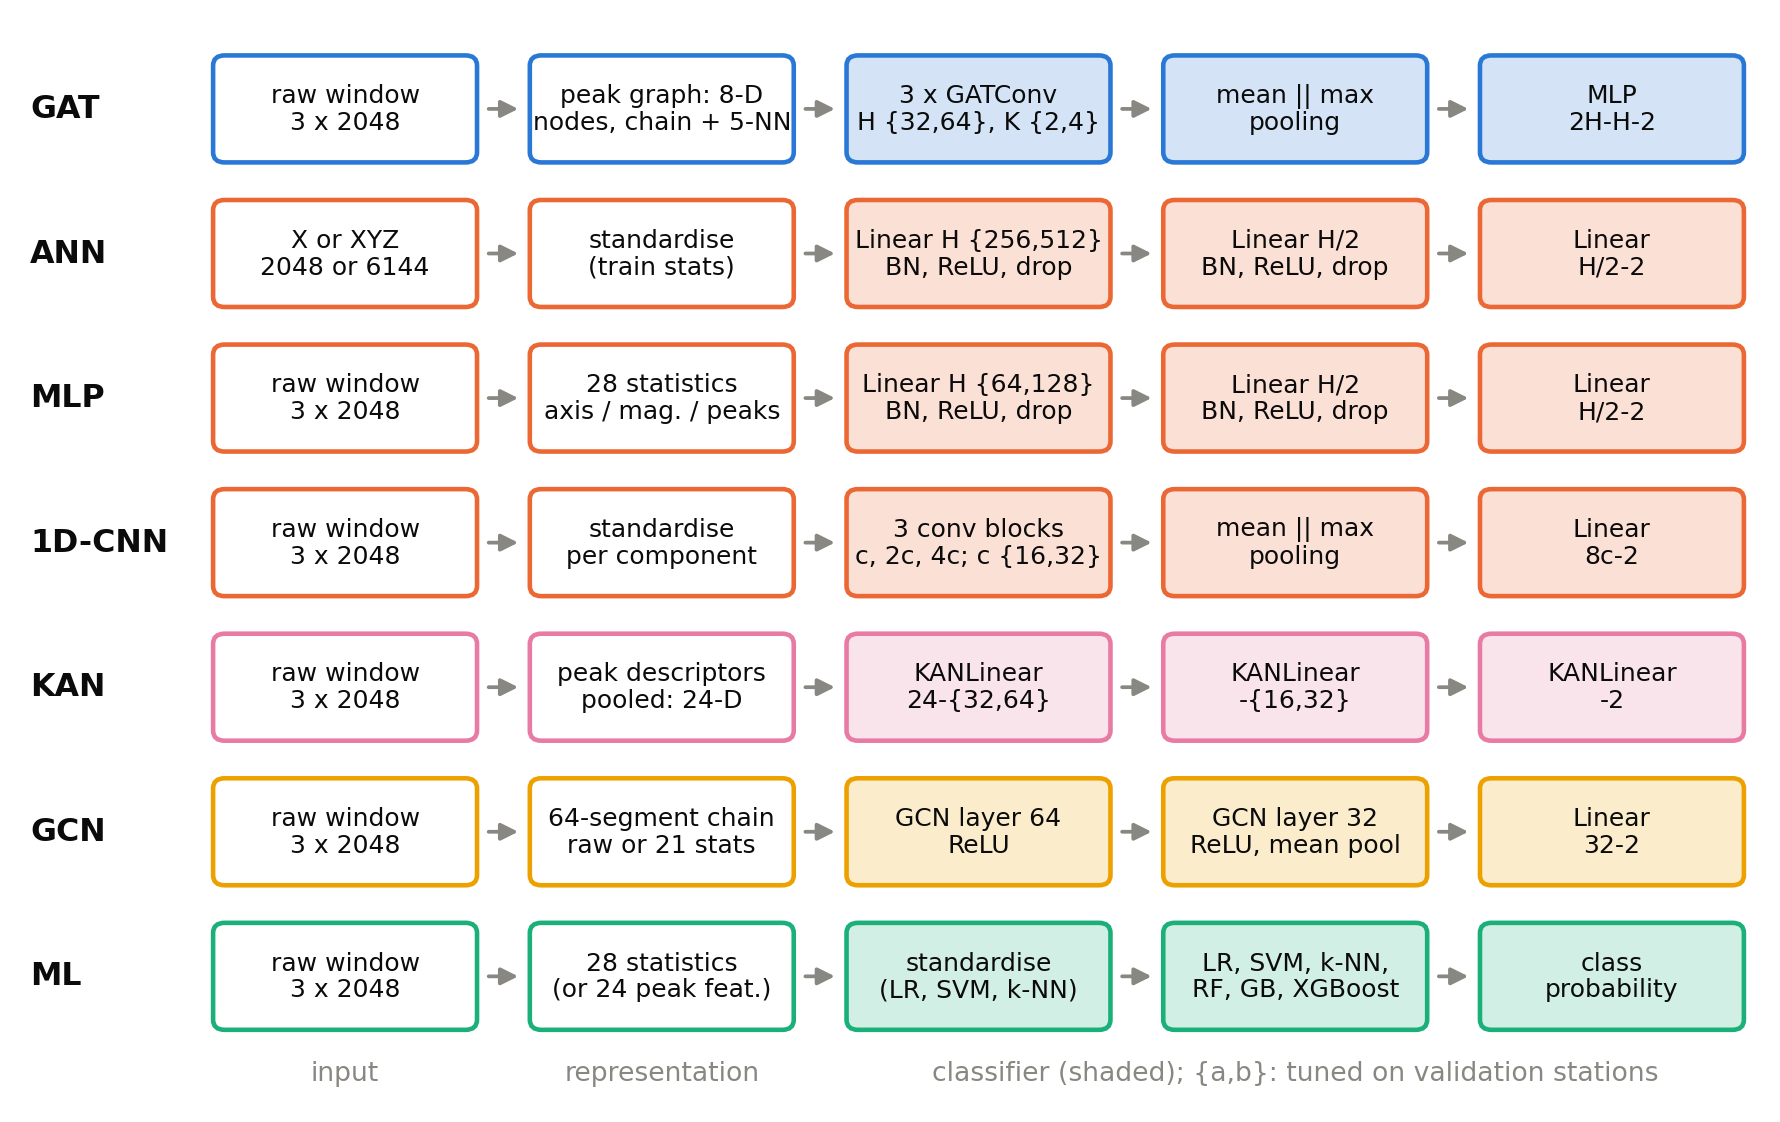
\includegraphics[width=0.92\textwidth]{figs/r_architectures.png}
\caption{The model pipelines of the benchmark. Each row runs left to right from the raw
window, through the representation the model consumes, to the classifier (shaded).
Values in braces are the alternatives searched on validation stations
(Table~\ref{tbl:tuning}). $H$, hidden width; $K$, attention heads; $c$, base number of
convolution channels.}
\label{fig:architectures}
\end{figure*}

\subsection{Evaluation protocol}\label{sec:protocol}
\paragraph{Station-held-out cross-validation.} The peak cohort is split by
\texttt{StratifiedGroupKFold} (scikit-learn; \citealp{pedregosa2011}) into five outer
folds with the station as the group, so every test fold consists of whole stations that
contribute no window to training or validation. Within each outer training set, a
second station-grouped split (one of four groups) is held out as the validation set.
Table~\ref{tbl:folds} lists the resulting partitions; every partition contains both
classes, and the code asserts that no station appears in both training and test data.

\begin{table}[width=\linewidth,cols=6,pos=t]
\caption{Station-held-out folds of the 54,901-window peak cohort: held-out stations and
window counts (test Giraffe windows in parentheses).}
\label{tbl:folds}
\footnotesize
\begin{tabular*}{\tblwidth}{@{}l@{\extracolsep{\fill}}lrlrr@{}}
\toprule
Fold & Test st. & Test & Val.\ st. & Val. & Train \\
\midrule
0 & 5, 12 & 11,197 (688) & 4, 11 & 15,368 & 28,336 \\
1 & 10, 18 & 8,622 (875) & 4, 11 & 15,368 & 30,911 \\
2 & 4, 19 & 14,284 (896) & 5, 16 & 10,459 & 30,158 \\
3 & 3 & 9,105 (506) & 10, 11 & 6,867 & 38,929 \\
4 & 11, 16, 17 & 11,693 (526) & 4, 5 & 19,242 & 23,966 \\
\bottomrule
\end{tabular*}
\end{table}

\paragraph{Selection and testing.} Every hyperparameter choice, every early-stopping
decision and every checkpoint uses validation balanced accuracy only; each test fold is
scored once, with the configuration chosen for that fold. Neural models train on the
training stations with early stopping on the validation stations. Classical estimators
are refitted on training plus validation stations with the selected setting. Each model
is run with seeds 0, 1 and 2; logistic regression, the SVM and $k$-NN are deterministic
and run once. Probabilities are thresholded at 0.5; no threshold is tuned.

\paragraph{Pooled and per-fold scores.} The five test folds of one seed together
predict every window of the cohort exactly once. Our primary score is the balanced
accuracy of these pooled out-of-fold predictions, averaged over seeds; we also report its
standard deviation over seeds, and the mean and standard deviation of the five per-fold
scores, which measure variation between held-out station groups.

\subsection{Peak-graph representation}\label{sec:peakgraph}
For each window, the three-component magnitude envelope is normalised within the
window:
\begin{equation}
\begin{aligned}
M(t)&=\sqrt{S_X(t)^2+S_Y(t)^2+S_Z(t)^2},\\
\tilde{M}(t)&=\frac{M(t)-\mu_M}{\sigma_M+\varepsilon}.
\end{aligned}
\end{equation}
Local maxima of $\tilde{M}$ are detected with prominence $\rho=0.05$ (in units of the
window's own standard deviation) and minimum separation $\delta=10$ samples (50\,ms).
Each peak becomes a node with eight features: the magnitude $M(t_i)$; the three raw
component values at $t_i$; the peak prominence; the sum of squared magnitude and its
standard deviation in a 20-sample window centred on the peak (clipped to the window
bounds); and the relative position $t_i/T$. Edges comprise bidirectional links between
successive peaks and directed 5-nearest-neighbour links in feature space, so a graph
with $N>5$ nodes has
\begin{equation}
E(N)=2(N-1)+5N=7N-2
\end{equation}
edges (152 for the 22-node example in Figure~\ref{fig:signal}). In the peak cohort a
graph has on average 64.5 nodes (median 52), i.e.\ 6.3 peaks per second, so nodes are
envelope maxima rather than individual footfalls. The raw node features differ in scale
by orders of magnitude (amplitudes and energies in sensor units, position in $[0,1]$);
whether to standardise them with training-fold statistics, which also changes the
nearest-neighbour edges, is a tuned choice (Table~\ref{tbl:tuning}).

\begin{figure*}[pos=t]
\centering
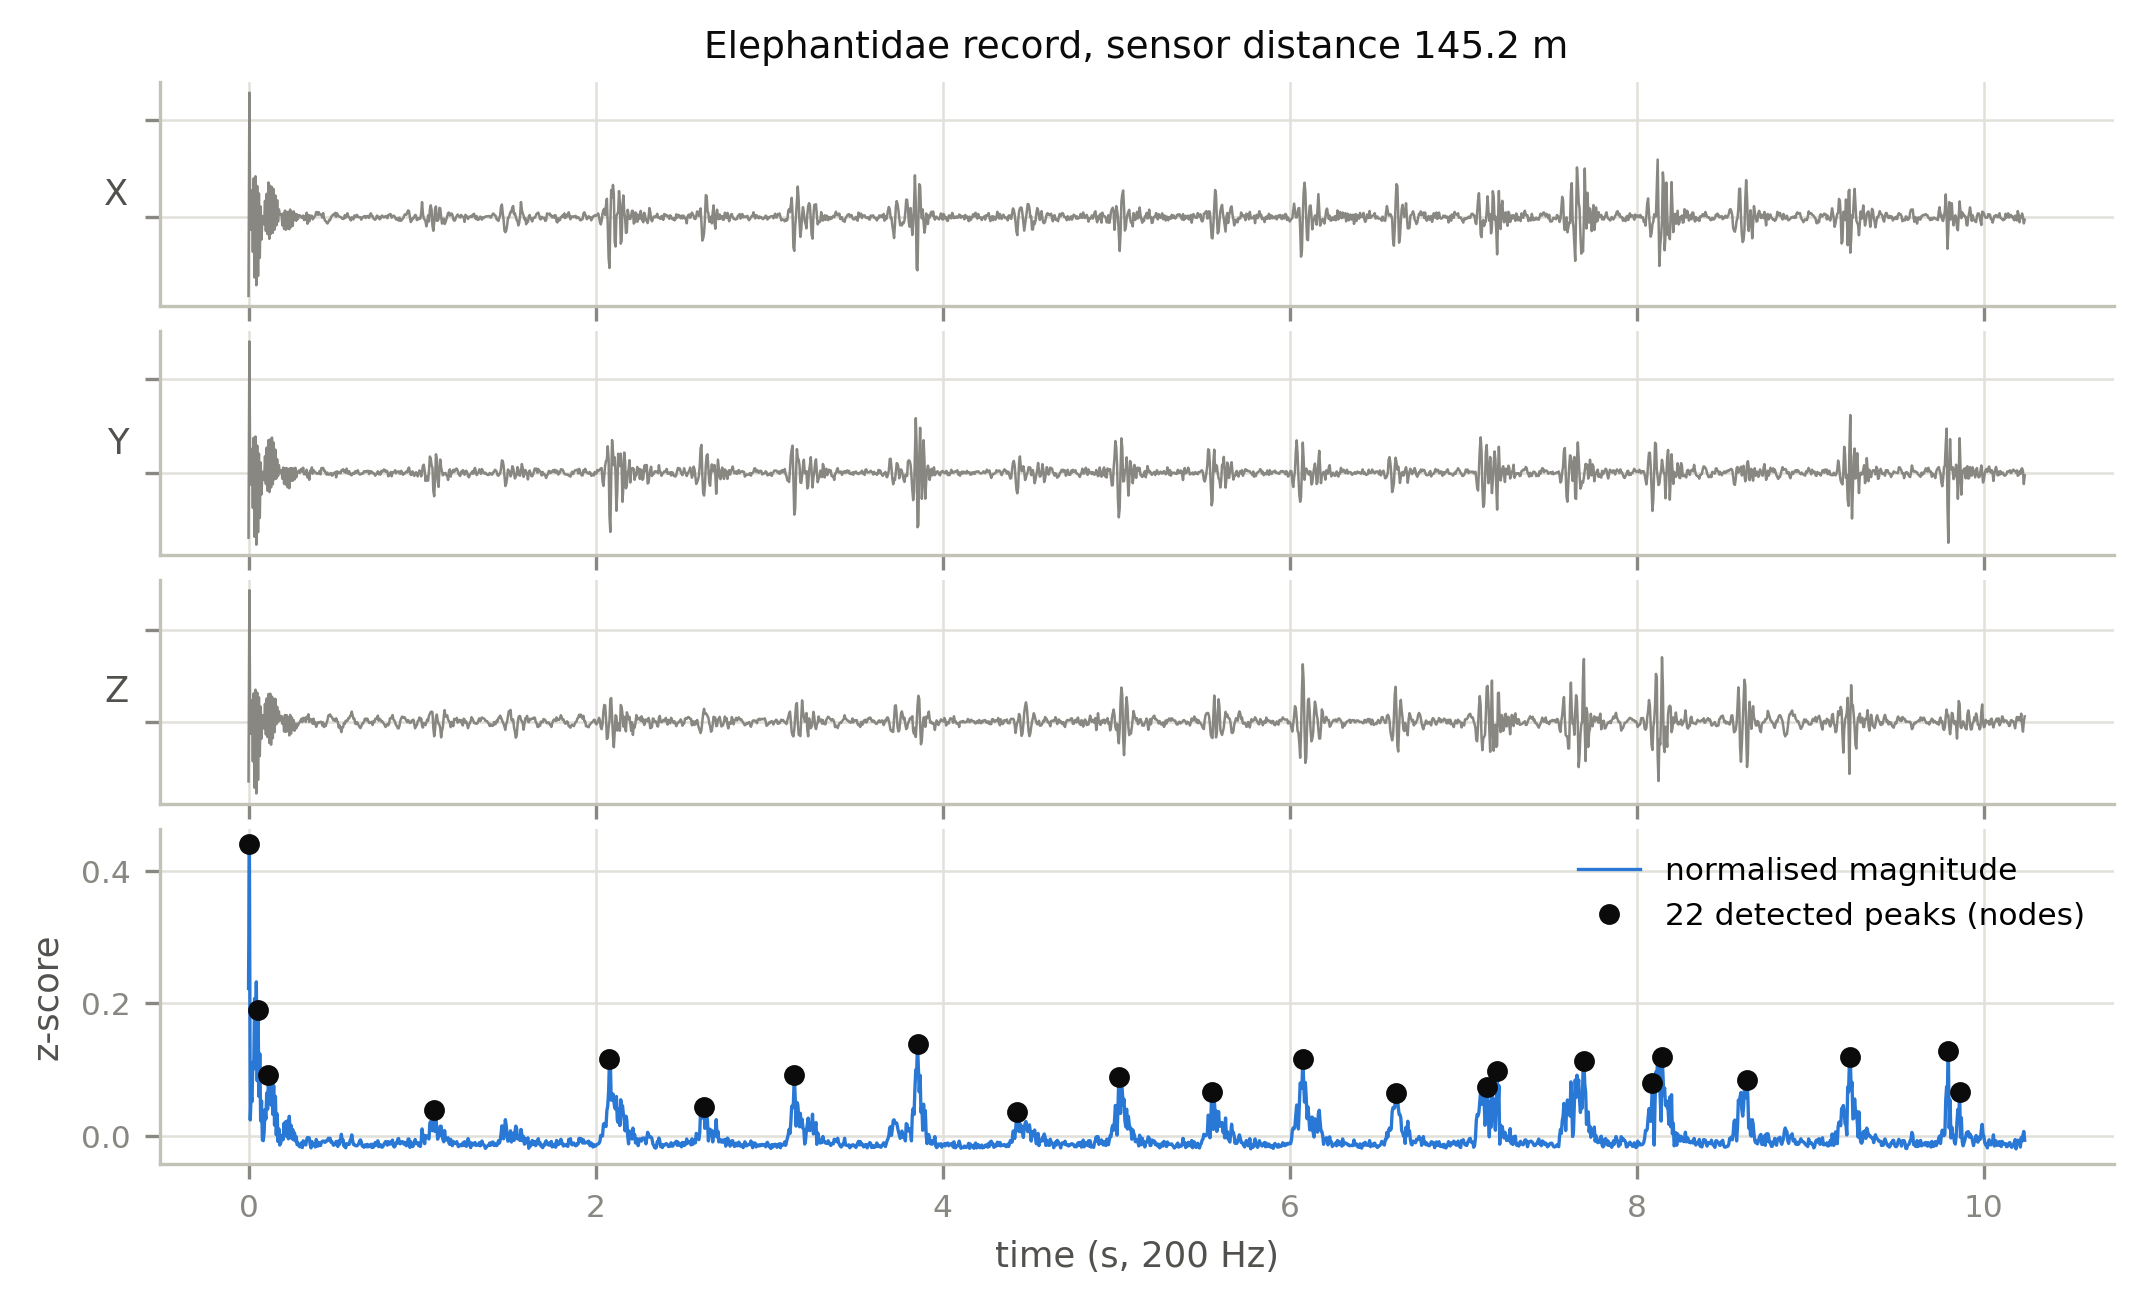
\includegraphics[width=0.92\textwidth]{figs/signal_and_peaks.png}
\caption{The first binary-task window in file order (Elephantidae, 145.2\,m): the three
raw components (top) and the per-window normalised magnitude envelope with the 22
detected peaks that become graph nodes (bottom; prominence 0.05, minimum separation
10 samples). Amplitude axes of the raw components are omitted because the data are
uncalibrated.}
\label{fig:signal}
\end{figure*}

\subsection{Graph Attention Network}\label{sec:gat}
For a node $i$ and neighbour $j$, graph attention \citep{velickovic2018} computes
\begin{align}
e_{ij}&=\mathrm{LeakyReLU}\!\left(\mathbf{a}^{\top}
      \left[\mathbf{W}\mathbf{x}_i \,\Vert\, \mathbf{W}\mathbf{x}_j\right]\right),\\
\alpha_{ij}&=\frac{\exp(e_{ij})}{\sum_{k\in\mathcal{N}(i)}\exp(e_{ik})},
\end{align}
with $K$ heads whose outputs are averaged:
\begin{equation}
\mathbf{h}_i'=\sigma\!\left(\frac{1}{K}\sum_{k=1}^{K}
   \sum_{j\in\mathcal{N}(i)}\alpha_{ij}^{\,k}\,\mathbf{W}^{k}\mathbf{x}_j\right).
\end{equation}
Three graph-attention layers (PyTorch Geometric; \citealp{fey2019}) add a self-loop to
every node, use ELU after the first two layers and dropout ($p=0.4$) after each. Global
mean and max pooling are concatenated and fed to a $2H\!\rightarrow\!H\!\rightarrow\!2$
classifier with batch normalisation, ReLU and dropout. With input width $F=8$ the number
of trainable parameters is
\begin{equation}
\begin{aligned}
P(H,K)=\;&\underbrace{(F+2H)KH+3(2KH+H)}_{\text{three GAT layers}}\\
&+\underbrace{2H^2+5H+2}_{\text{classifier}},
\end{aligned}
\end{equation}
i.e.\ 7,298 to 45,058 over the searched widths and head counts. Training uses Adam,
batch size 64, weight decay $10^{-4}$ and at most 100 epochs with early-stopping
patience 15.

\subsection{Neural baselines}\label{sec:nn}
\paragraph{ANN.} A dense network classifies the standardised raw waveform, either the X
component alone (2,048 values) or all three components (6,144 values), through
$H\rightarrow H/2\rightarrow2$ layers with batch normalisation, ReLU and dropout 0.5
($H\in\{256,512\}$; 0.56 to 3.28 million parameters). It has no temporal inductive bias
and serves as the naive raw-signal baseline.

\paragraph{Feature MLP.} The same architecture ($H\in\{64,128\}$) is applied to the 28
standardised engineered features of Section~\ref{sec:ml}, separating the effect of the
network from that of the input.

\paragraph{1D-CNN.} A compact convolutional network on the three standardised components
uses three blocks of convolution (kernel 9), batch normalisation and ReLU with $c$, $2c$
and $4c$ channels (stride 2 in the first block, max pooling by 4 after the first two),
concatenated global mean and max pooling, dropout 0.3 and a linear output
($c\in\{16,32\}$; 24,066 or 94,210 parameters).

\paragraph{KAN.} A Kolmogorov--Arnold network \citep{liu2024kan} classifies the 24
standardised statistics obtained by pooling the eight peak descriptors over the $P$
peaks of a window,
\begin{equation}
\mathbf{z}=\left[\operatorname{mean}_{i}(\mathbf{x}_i),\;
\operatorname{max}_{i}(\mathbf{x}_i),\;
\operatorname{std}_{i}(\mathbf{x}_i)\right]\in\mathbb{R}^{24}.
\end{equation}
Each KANLinear layer combines a SiLU base map with a learned cubic B-spline map over five
grid intervals,
\begin{equation}
\operatorname{KANLinear}(\mathbf{x})=
\mathbf{W}_{b}\,\operatorname{SiLU}(\mathbf{x})+
\mathbf{W}_{s}\,\mathbf{B}(\mathbf{x}),
\end{equation}
with widths $24\rightarrow32\rightarrow16\rightarrow2$ or
$24\rightarrow64\rightarrow32\rightarrow2$, dropout 0.1 between layers and gradient-norm
clipping at 1.

\paragraph{GCN.} Each window, standardised per component with training statistics, is cut
into 64 contiguous 32-sample segments (0.16\,s) that form a chain graph with self-loops.
Node features are either the 96 raw values of a segment or 21 standardised statistics
(mean, standard deviation, minimum, maximum, root-mean-square, sum of squares and range
per component). Two graph-convolution layers \citep{kipf2017},
\begin{equation}
\mathbf{H}^{(\ell+1)}=\mathrm{ReLU}\!\left(
\tilde{\mathbf{D}}^{-1/2}\tilde{\mathbf{A}}\tilde{\mathbf{D}}^{-1/2}
\mathbf{H}^{(\ell)}\mathbf{W}^{(\ell)}\right),
\end{equation}
map to 64 and 32 channels (with batch normalisation and dropout 0.3 for the statistics
encoding), followed by mean pooling and a linear output.

All neural baselines use Adam, weight decay $10^{-4}$, batch size 128, at most 60 epochs
and early-stopping patience 10.

\subsection{Classical machine learning}\label{sec:ml}
The classical pipeline computes 28 features per window: six statistics per raw
component (mean, standard deviation, maximum, absolute maximum, sum of squares and
zero-crossing rate); four magnitude statistics (mean, standard deviation, maximum and
sum of squares); and six peak statistics (count, mean, standard deviation and maximum of
peak height, mean prominence and mean inter-peak gap). Six estimators are compared:
logistic regression, an RBF-kernel support vector machine (SVM), $k$-nearest neighbours
($k$-NN), a 300-tree random forest, a 200-stage gradient-boosting classifier
(scikit-learn; \citealp{pedregosa2011}) and 300-tree XGBoost \citep{chen2016xgboost}.
Logistic regression, the SVM and $k$-NN use features standardised on the training data.

Two further XGBoost variants answer specific questions. \emph{XGBoost (peak features)}
uses the 24 pooled peak descriptors of the KAN: it sees the same information as the GAT
without a graph and is the graph-free baseline of Section~\ref{sec:ablation-method}.
\emph{XGBoost [all windows]} uses the 28 features on all 66,814 binary windows with its
own station-held-out folds, and, with an ANN on the same windows, checks the effect of the
peak-cohort restriction.

\subsection{Imbalance handling}\label{sec:weight}
Neural models minimise weighted cross-entropy,
\begin{equation}
\mathcal{L}=-\frac{\sum_{n}w_{y_n}\log p_\theta(y_n\mid x_n)}{\sum_n w_{y_n}},\qquad
w_c=\frac{N}{2N_c},
\end{equation}
with class counts $N_c$ from the training stations of each fold. Logistic regression,
the SVM and the random forest use balanced class weights, gradient boosting balanced
sample weights, and XGBoost a positive-class weight equal to the training class ratio;
$k$-NN is unweighted.

\subsection{Hyperparameter search}\label{sec:tuning}
Table~\ref{tbl:tuning} lists the grids. Each configuration is trained once per outer
fold (seed 0) and scored on that fold's validation stations; the best configuration is
then trained with three seeds. The GAT grid (16 configurations, at most 20 epochs with
patience 5 during the search) is the largest; the neural baselines have 4 or 8
configurations and the classical estimators 1 to 6. Exhaustive grids are adequate for
these small, discrete spaces \citep{bergstra2012}.

\begin{table*}[width=.98\textwidth,cols=4,pos=t]
\caption{Hyperparameter grids, searched separately in every outer fold on validation
stations only, and the configurations selected across the five folds.}\label{tbl:tuning}
\footnotesize
\begin{tabular*}{\tblwidth}{@{}p{2.4cm}p{6.4cm}r@{\extracolsep{\fill}}p{6.0cm}@{}}
\toprule
Model & Grid & Size & Selected in the five folds \\
\midrule
GAT & $H\in\{32,64\}$ $\times$ $K\in\{2,4\}$ $\times$ lr $\{10^{-3},5{\times}10^{-4}\}$
$\times$ node features \{raw, standardised\} & 16 & raw features in 5/5; $H=64$ in 4/5;
$K=2$ in 3/5 \\
ANN & input \{X, XYZ\} $\times$ $H\in\{256,512\}$ $\times$ lr $\{10^{-3},10^{-4}\}$ & 8 &
XYZ in 4/5; $H=512$ in 3/5 \\
Feature MLP & $H\in\{64,128\}$ $\times$ lr $\{10^{-3},5{\times}10^{-4}\}$ & 4 & $H=64$ in
3/5 \\
1D-CNN & $c\in\{16,32\}$ $\times$ lr $\{10^{-3},5{\times}10^{-4}\}$ & 4 & $c=32$ in 4/5 \\
KAN & widths \{32--16, 64--32\} $\times$ lr $\{10^{-3},5{\times}10^{-4}\}$ & 4 & 32--16 in
4/5 \\
GCN & node encoding \{raw segment, 21 statistics\} $\times$ lr
$\{10^{-3},5{\times}10^{-4}\}$ & 4 & statistics, lr $10^{-3}$ in 5/5 \\
Logistic reg. & $C\in\{0.1,1,10\}$ & 3 & $C=10$ in 4/5 \\
SVM (RBF) & $C\in\{1,10\}$ & 2 & $C=1$ in 4/5 \\
$k$-NN & $k\in\{7,15\}$ $\times$ weights \{uniform, distance\} & 4 & $k=15$ in 3/5 \\
Random forest & max.\ depth \{none, 20\} & 2 & depth 20 in 3/5 \\
Grad.\ boosting & learning rate 0.1 & 1 & --- \\
XGBoost & max.\ depth $\{3,5,7\}$ $\times$ lr $\{0.05,0.1\}$ & 6 & depth 3 in 3/5 \\
\bottomrule
\end{tabular*}
\end{table*}

\subsection{Graph ablations, attention and detector sensitivity}\label{sec:ablation-method}
\paragraph{Graph ablations.} With the configuration selected for each fold, the GAT is
retrained (seed 0) with (a) temporal edges only, (b) nearest-neighbour edges only,
(c) the same number of edges between uniformly random node pairs, (d) no edges (each
node sees only itself), and (e) the other node-scaling option. Ablation (d) reduces the
GAT to a per-node network with pooling; together with XGBoost on pooled peak features,
it separates the value of the peak features from that of message passing and of the
specific edge structure.

\paragraph{Attention faithfulness.} For each fold's seed-0 GAT, we score up to 2,000
test graphs, rank nodes by the attention they send to other nodes (averaged over heads
and summed over layers), delete the top 10, 25 or 50\% of nodes or the same number of
random nodes, and record the fraction of predictions that change and the balanced
accuracy after deletion. Attention identifies influential nodes if top-attention deletion
changes predictions more than random deletion \citep{jain2019}.

\paragraph{Detector sweep.} Peak detection is re-run with prominence
$\rho\in\{0.05,0.1,0.25,0.5\}$ and minimum separation $\delta\in\{10,40\}$ samples
(50 or 200\,ms). For each setting we record the fraction of windows of each class that
keep at least two peaks, the graph size, and the balanced accuracy of XGBoost (depth 5,
learning rate 0.1) on the pooled peak features under the same station-held-out protocol.

\subsection{Metrics and uncertainty}\label{sec:metrics}
With Giraffe as the positive class, the confusion matrix has entries TP, FP, FN and TN.
We report
\begin{align}
\mathrm{BA}&=\tfrac12\!\left(\tfrac{\mathrm{TP}}{\mathrm{TP}+\mathrm{FN}}
+\tfrac{\mathrm{TN}}{\mathrm{TN}+\mathrm{FP}}\right),\\
\mathrm{MCC}&=\frac{\mathrm{TP}\cdot\mathrm{TN}-\mathrm{FP}\cdot\mathrm{FN}}
{\sqrt{(\mathrm{TP}{+}\mathrm{FP})(\mathrm{TP}{+}\mathrm{FN})(\mathrm{TN}{+}\mathrm{FP})(\mathrm{TN}{+}\mathrm{FN})}},
\end{align}
macro-F1, Giraffe precision and recall, and the threshold-free areas under the ROC
(AUROC) and precision--recall (AUPRC) curves; the AUPRC of a random classifier equals the
Giraffe share, 0.064. Balanced accuracy is the primary metric because it equals 0.5 for
any constant predictor \citep{brodersen2010}, and MCC is high only when all four cells
are good \citep{chicco2020}. Accuracy is reported only to show how it misleads.

Windows recorded at one station during one animal passage are not independent, so
tests that treat windows as independent observations overstate significance. We
computed McNemar's test with Holm correction on the pooled seed-0 predictions of all 78
model pairs; with 54,901 dependent windows, all pairs but one were ``significant'',
which reflects sample size rather than meaningful differences. We therefore judge
differences against the variation between held-out station groups (fold standard
deviation) and between seeds, and avoid claims of significance.

\subsection{Comparison with random splits}\label{sec:random-method}
To quantify how much the earlier, random-split results were inflated, we compare them
with the station-held-out results for the eight models that exist in both. The earlier
models were trained on a stratified random 80/20 split of windows (seed 42) and selected
on the test partition; the GAT used the peak cohort and the other models all binary
windows. As a direct control that changes only the split, the benchmark code re-runs
XGBoost, logistic regression and the earlier GAT configuration ($H=64$, $K=4$, raw
features, learning rate $10^{-3}$) under the same protocol but with stratified random
window-level folds. % TODO: add the control results to Section 5.4 when they arrive.

\subsection{Edge profiling}\label{sec:edge-method}
The deployment target is an ESP32-S3 microcontroller (dual-core Xtensa LX7 at up to
240\,MHz, 512\,KB of on-chip SRAM, 4--16\,MB of flash). Following common tiny-ML practice
\citep{banbury2021}, we adopt budgets of at most 512\,KB of stored model and 200\,KB of
working memory. For the fold-0, seed-0 model of each family we measure the parameter
count, the serialised FP32 size and the size after PyTorch dynamic INT8 quantisation
\citep{jacob2018}, which quantises linear layers only. For tree ensembles we count split
and leaf nodes and compute the size of the trees as flat C arrays (a 4-byte threshold,
a 1-byte feature index and two 2-byte child indices per split; a 4-byte value per leaf).
Latency is measured on the host CPU with one thread, as the median over 200 test windows
of the best of three repetitions, separately for preprocessing (feature extraction or
graph construction) and inference. Host latencies are a relative measure only; no model
was run on the device, so on-device latency and energy remain unmeasured. For the GAT we
also derive working memory and multiply--accumulate (MAC) operations from the graph size.

\subsection{Computing environment}\label{sec:env}
Experiments ran on an NVIDIA DGX server (A100-SXM4-80GB GPUs, 256 CPU cores) with
Python 3.9.16, PyTorch 2.8.0, PyTorch Geometric 2.6.1, scikit-learn 1.3.2, XGBoost 2.1.4,
SciPy 1.11.4 and NumPy 1.26.4. Because the benchmark consists of many small, independent
training runs, a job scheduler ran two worker processes per free GPU, each taking jobs
(one model, fold, seed and configuration) from a shared queue; the 423 jobs of the main
benchmark finished in about 50\,min. The script, configuration and every per-run result
and prediction file are released (see Data availability).

\section{Results}\label{sec:results}

\subsection{Station-held-out comparison (RQ1)}\label{sec:res-main}
Table~\ref{tbl:main} and Figure~\ref{fig:main} report all thirteen classifiers. Every
classifier was weak on unseen stations: pooled balanced accuracy ranged from 0.526
($k$-NN) to 0.603 (logistic regression), MCC from 0.028 to 0.114 and AUROC from 0.536 to
0.621, and no model recovered Giraffe windows at a precision above 0.21. The four best
models used whole-window information: logistic regression (0.603), XGBoost (0.590) and
the feature MLP (0.573) on the 28 engineered features, and the 1D-CNN (0.585) on the raw
components. The graph models were in the middle and lower part of the ranking (GAT
0.559, GCN 0.528), as was the KAN (0.544).

\begin{table*}[width=.98\textwidth,cols=11,pos=t]
\caption{Station-held-out results on the 54,901-window peak cohort (Giraffe positive;
sorted by pooled balanced accuracy). BA: balanced accuracy of the pooled out-of-fold
predictions, mean (standard deviation) over seeds; Fold BA: mean $\pm$ standard deviation
over the five held-out station groups. Other metrics are pooled means over seeds. Rows
below the line use all 66,814 binary windows. Deterministic estimators were run once.}
\label{tbl:main}
\footnotesize
\begin{tabular*}{\tblwidth}{@{}l@{\extracolsep{\fill}}llrrrrrrr@{}}
\toprule
Model & BA (seed SD) & Fold BA & MCC & Macro-F1 & Accuracy & Gir.\ P & Gir.\ R & AUROC & AUPRC \\
\midrule
Logistic reg. & \textbf{0.603} (---) & 0.606 $\pm$ 0.078 & 0.103 & 0.463 & 0.630 & 0.096 & \textbf{0.571} & 0.611 & 0.104 \\
XGBoost & 0.590 (0.000) & 0.591 $\pm$ 0.051 & \textbf{0.114} & 0.535 & 0.802 & 0.123 & 0.346 & \textbf{0.621} & 0.114 \\
1D-CNN & 0.585 (0.046) & 0.586 $\pm$ 0.041 & 0.100 & 0.510 & 0.744 & 0.109 & 0.403 & 0.603 & \textbf{0.142} \\
Feature MLP & 0.573 (0.008) & 0.576 $\pm$ 0.043 & 0.082 & 0.494 & 0.720 & 0.098 & 0.405 & 0.594 & 0.109 \\
SVM (RBF) & 0.561 (---) & 0.563 $\pm$ 0.051 & 0.070 & 0.499 & 0.744 & 0.094 & 0.352 & 0.580 & 0.105 \\
GAT & 0.559 (0.019) & 0.541 $\pm$ 0.023 & 0.068 & 0.496 & 0.736 & 0.094 & 0.356 & 0.577 & 0.096 \\
Random forest & 0.553 (0.001) & 0.554 $\pm$ 0.030 & 0.083 & \textbf{0.537} & 0.854 & 0.122 & 0.208 & 0.590 & 0.093 \\
ANN & 0.551 (0.006) & 0.543 $\pm$ 0.015 & 0.066 & 0.515 & 0.798 & 0.099 & 0.267 & 0.545 & 0.088 \\
KAN & 0.544 (0.004) & 0.533 $\pm$ 0.064 & 0.049 & 0.486 & 0.726 & 0.084 & 0.336 & 0.536 & 0.071 \\
XGBoost (peak features) & 0.543 (0.000) & 0.537 $\pm$ 0.044 & 0.049 & 0.486 & 0.728 & 0.084 & 0.332 & 0.572 & 0.082 \\
Grad.\ boosting & 0.542 (0.002) & 0.554 $\pm$ 0.048 & 0.043 & 0.462 & 0.666 & 0.079 & 0.400 & 0.556 & 0.083 \\
GCN & 0.528 (0.004) & 0.545 $\pm$ 0.044 & 0.028 & 0.410 & 0.548 & 0.071 & 0.506 & 0.563 & 0.103 \\
$k$-NN & 0.526 (---) & 0.528 $\pm$ 0.020 & 0.088 & 0.533 & \textbf{0.924} & \textbf{0.209} & 0.070 & 0.591 & 0.095 \\
\midrule
XGBoost [all windows] & 0.583 (0.000) & 0.582 $\pm$ 0.055 & 0.091 & 0.495 & 0.713 & 0.101 & 0.434 & 0.599 & 0.105 \\
ANN [all windows] & 0.528 (0.004) & 0.516 $\pm$ 0.017 & 0.031 & 0.469 & 0.696 & 0.078 & 0.334 & 0.501 & 0.083 \\
\bottomrule
\end{tabular*}
\end{table*}

\begin{figure}[pos=t]
\centering
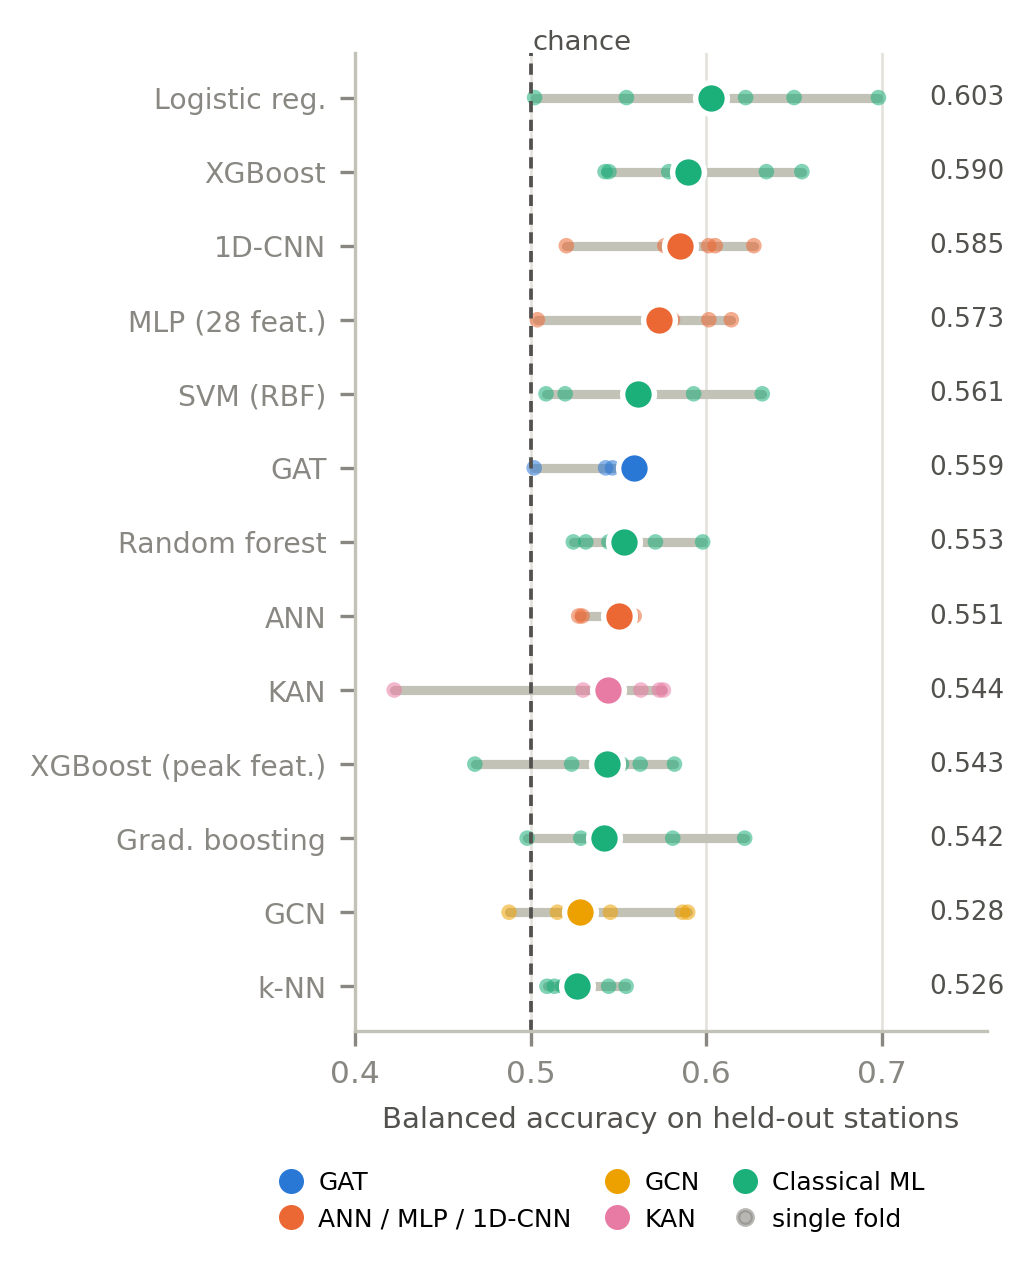
\includegraphics[width=\columnwidth]{figs/r_main_comparison.png}
\caption{Balanced accuracy on held-out stations. Large dots: pooled out-of-fold balanced
accuracy (mean over seeds, value at right); small dots and grey bar: the five held-out
station groups (mean over seeds) and their range. The dashed line marks chance.}
\label{fig:main}
\end{figure}

\paragraph{Differences between models are small relative to differences between stations.}
The pooled scores of the top five models lie within 0.04 of one another, whereas the
balanced accuracy of a single model varied by up to 0.20 between held-out station groups
(logistic regression: 0.502 on stations 11, 16 and 17; 0.698 on station 3;
Figure~\ref{fig:folds}). The ranking also changed between folds: XGBoost was best on fold
0 (0.655), logistic regression on folds 1--3, and on fold 4 no model exceeded 0.57.
Seed variation was small for most models but not for the 1D-CNN (seed standard deviation
0.046). The ranking of logistic regression above XGBoost, the 1D-CNN and the feature MLP
is therefore not established; what is established is that all four are of similar,
modest accuracy and that the remaining models are not better.

\begin{figure}[pos=t]
\centering
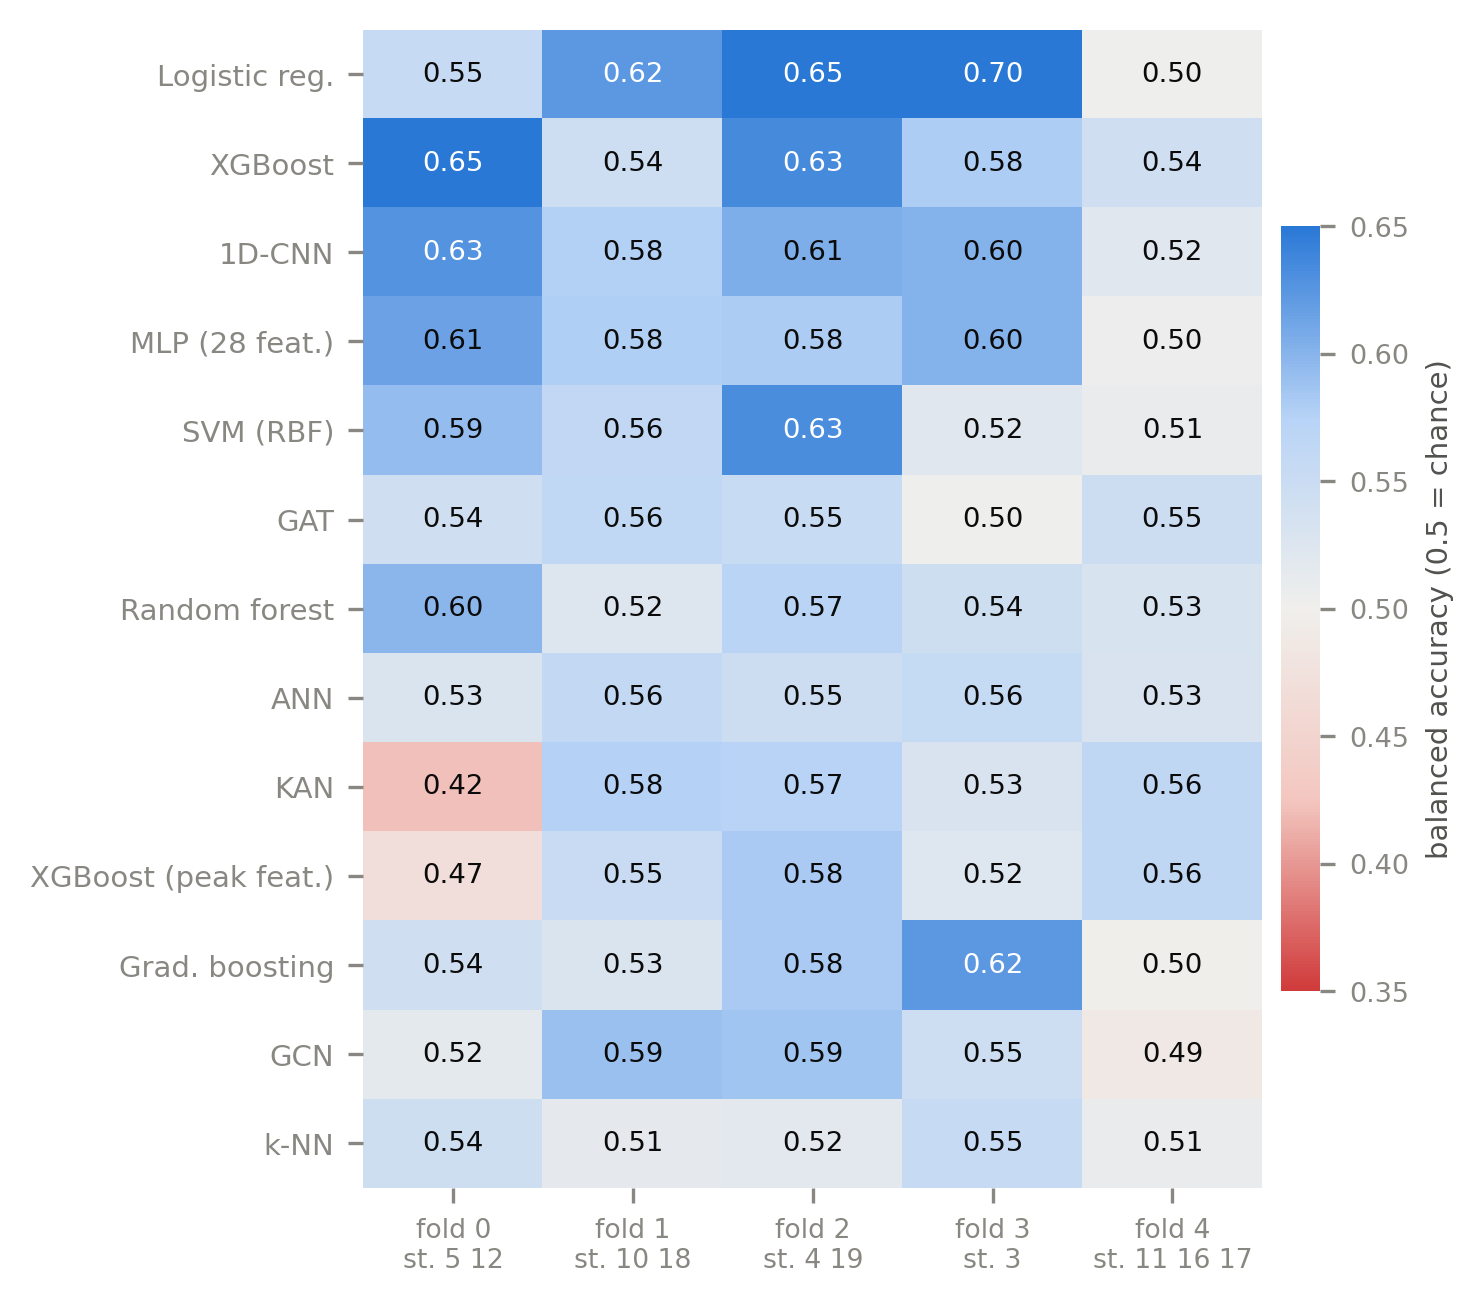
\includegraphics[width=\columnwidth]{figs/r_fold_heatmap.png}
\caption{Balanced accuracy of each model (rows) on each held-out station group (columns;
mean over seeds). Blue is above chance, red below.}
\label{fig:folds}
\end{figure}

\paragraph{Accuracy is misleading.} $k$-NN had the highest accuracy (0.924) and Giraffe
precision (0.209) but recovered only 7.0\% of Giraffe windows, giving the lowest balanced
accuracy; logistic regression had the lowest accuracy among the strong models (0.630)
because it recovered 57.1\% of Giraffe windows at the cost of many false alarms. Accuracy
reverses the ranking of these two models, and macro-F1, which rewards the majority class,
placed the random forest and $k$-NN among its top three. Balanced accuracy and AUROC
agreed on the leading group; MCC, which rewards precision, ranked $k$-NN mid-table.

\paragraph{Cohort restriction.} XGBoost on all 66,814 windows reached 0.583, against
0.590 on the peak cohort, and the ANN 0.528 against 0.551, so restricting the comparison
to windows with at least two peaks does not change the conclusions.

\subsection{Station shift and model selection (RQ3)}\label{sec:res-shift}
Figure~\ref{fig:valtest} relates the validation balanced accuracy of each selected
model to its test balanced accuracy in the same fold. Across the 65 model--fold pairs
the correlation was $r=-0.02$: performance on the validation stations did not predict
performance on the test stations. Gradient boosting on fold 3, for example, scored 0.334
on its validation stations and 0.622 on its test station. Consistent with this,
validation-based early stopping retained the first or second epoch in 23 of the 90 neural
runs (Figure~\ref{fig:curves}): validation balanced accuracy peaked early and then fluctuated
while the training loss continued to fall, as expected when what a model learns about
the training stations does not transfer to others.

\begin{figure}[pos=t]
\centering
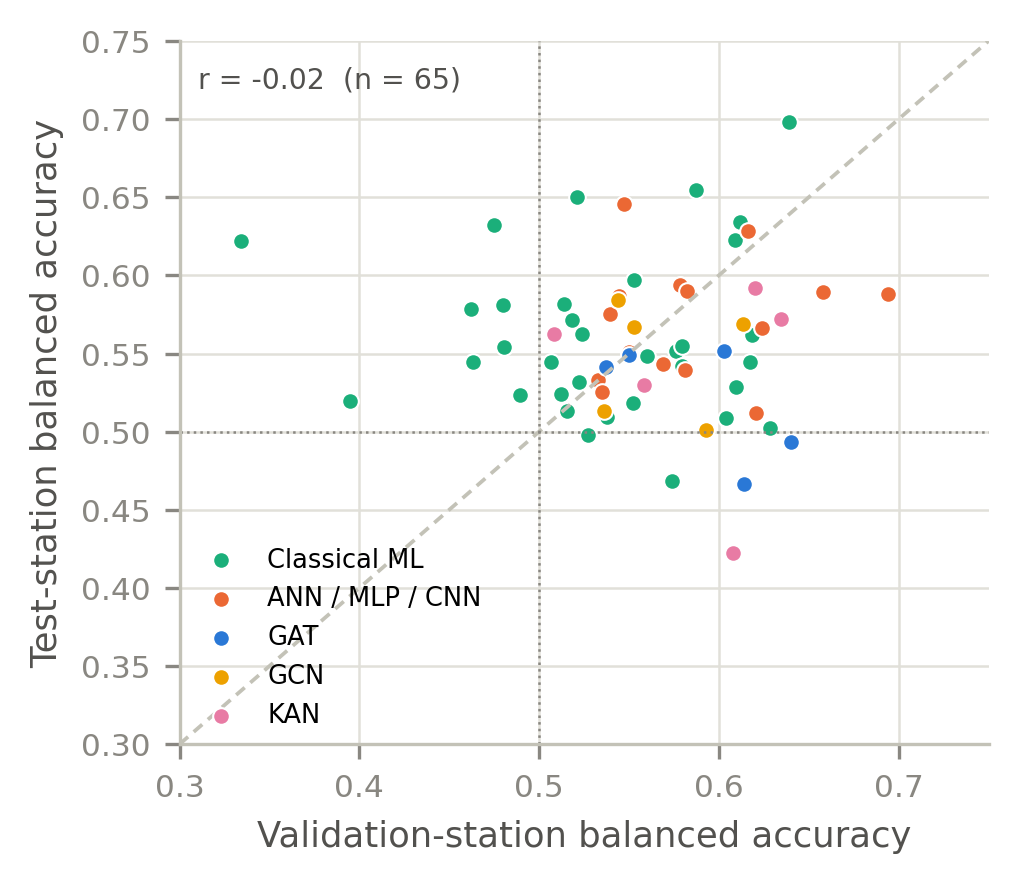
\includegraphics[width=\columnwidth]{figs/r_val_vs_test.png}
\caption{Validation-station against test-station balanced accuracy of the selected
configuration of every model in every fold (seed 0). The dashed diagonal marks equality;
dotted lines mark chance.}
\label{fig:valtest}
\end{figure}

\begin{figure*}[pos=t]
\centering
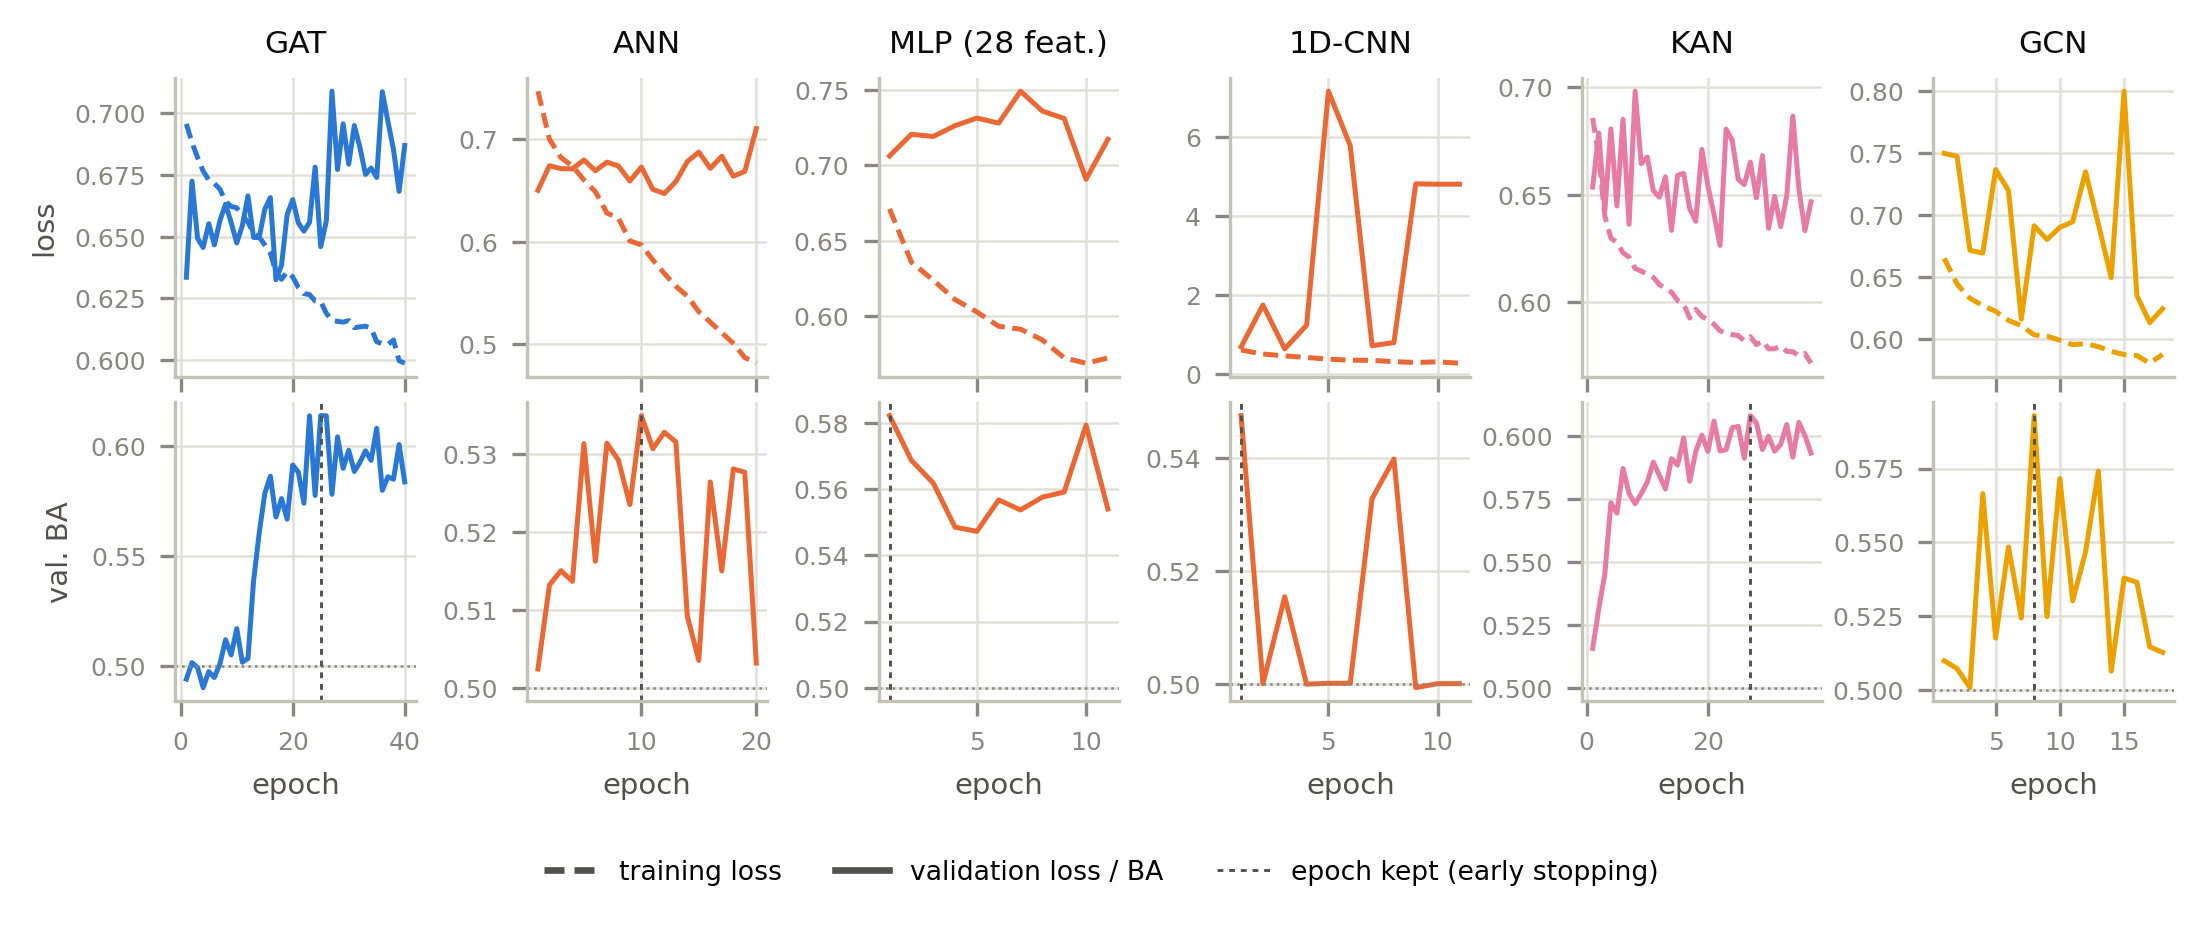
\includegraphics[width=0.98\textwidth]{figs/r_training_curves.png}
\caption{Training curves of the six neural models (fold 0, seed 0). Top: weighted
training and validation loss; bottom: validation balanced accuracy, with the epoch kept
by early stopping (dashed vertical line) and chance (dotted).}
\label{fig:curves}
\end{figure*}

\paragraph{Hyperparameter sensitivity.} Within each fold, the 16 GAT configurations
differed modestly in validation balanced accuracy (fold ranges 0.035--0.105), and the
fold accounted for most of the variation (fold means 0.517--0.628). Averaged over folds,
width 64 scored 0.016 above width 32, two heads 0.007 above four, and standardised node
features 0.007 above raw ones, although the single best configuration used raw features
in every fold. For the GCN, raw segments scored at chance on validation stations (0.500)
against 0.559 for segment statistics, which were selected in every fold. The other grids
had effects below 0.02 (ANN: X versus XYZ input, 0.536 versus 0.538). Because validation
scores did not predict test scores, these differences should not be read as transferable
tuning gains.

\subsection{Does the graph help? (RQ2)}\label{sec:res-graph}
Figure~\ref{fig:ablation} compares the GAT with its ablations and with XGBoost on the
pooled peak features. Removing all edges reduced pooled balanced accuracy from 0.559 to
0.523 and the fold mean from 0.541 to 0.498, so exchanging information between peaks
helps. Which peaks are connected did not matter: random edges (0.564) matched the
structured graph, while temporal-only (0.533) and nearest-neighbour-only edges (0.533)
were slightly lower. Standardising the node features gave 0.568. The ablations were run
with one seed and the GAT's seed standard deviation was 0.019, so only the no-edge
result stands out from seed variation. Without any graph, XGBoost on the 24 pooled peak
features reached 0.543, close to the GAT; XGBoost on the 28 whole-window features
reached 0.590. The peak representation, rather than the choice between graph and
graph-free models, therefore limits the peak-based models.

\begin{figure}[pos=t]
\centering
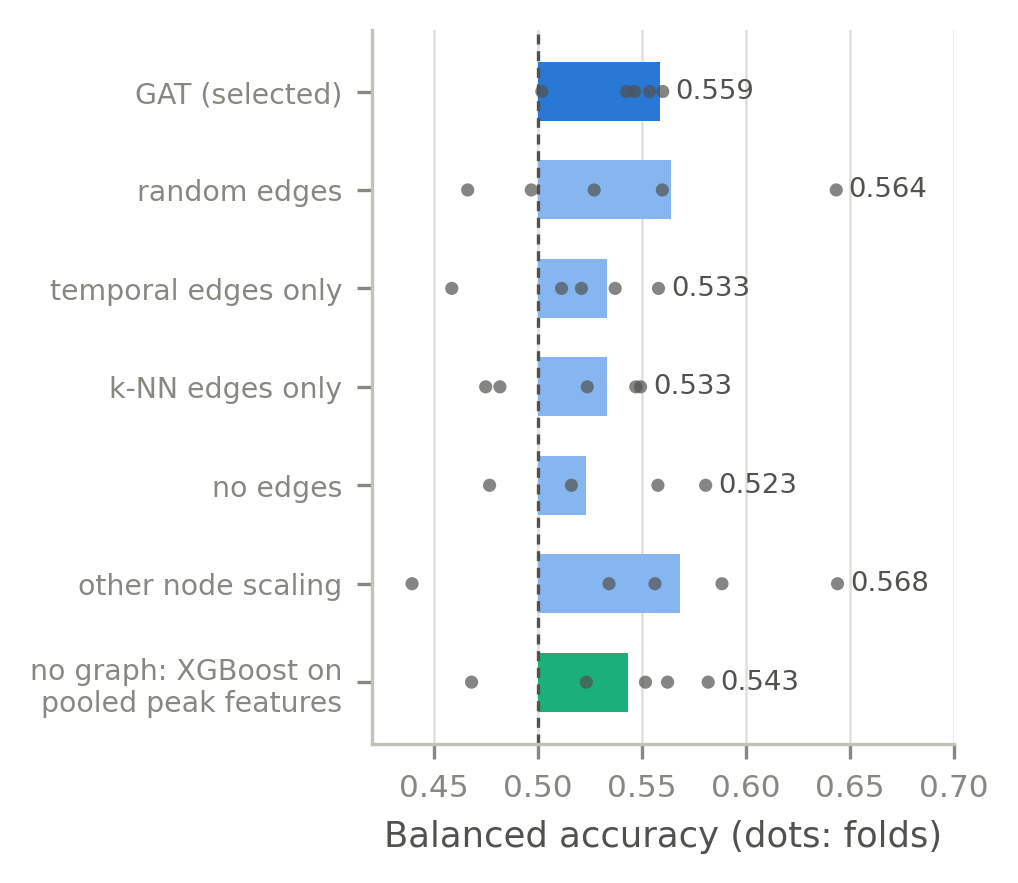
\includegraphics[width=\columnwidth]{figs/r_graph_ablation.png}
\caption{GAT graph ablations (pooled balanced accuracy; dots, the five held-out station
groups) and XGBoost on the pooled peak features. The selected GAT uses three seeds, the
ablations one.}
\label{fig:ablation}
\end{figure}

\paragraph{Attention faithfulness.} Deleting the nodes that sent the most attention
changed more predictions than deleting the same number of random nodes: 16.2\% against
6.2\% at 10\% deletion, 21.1\% against 11.8\% at 25\% and 24.0\% against 19.5\% at 50\%
(Figure~\ref{fig:attention}a; means over folds). In every fold, top-attention deletion
changed more predictions than random deletion at 10\%. Balanced accuracy, however, did
not fall: it was 0.519 on the intact subsample and 0.526--0.533 after either deletion
(Figure~\ref{fig:attention}b). Attention therefore marks the nodes the model relies on,
but those nodes do not carry class evidence that transfers to unseen stations, and the
attention weights should not be interpreted as identifying diagnostic footfalls.

\begin{figure}[pos=t]
\centering
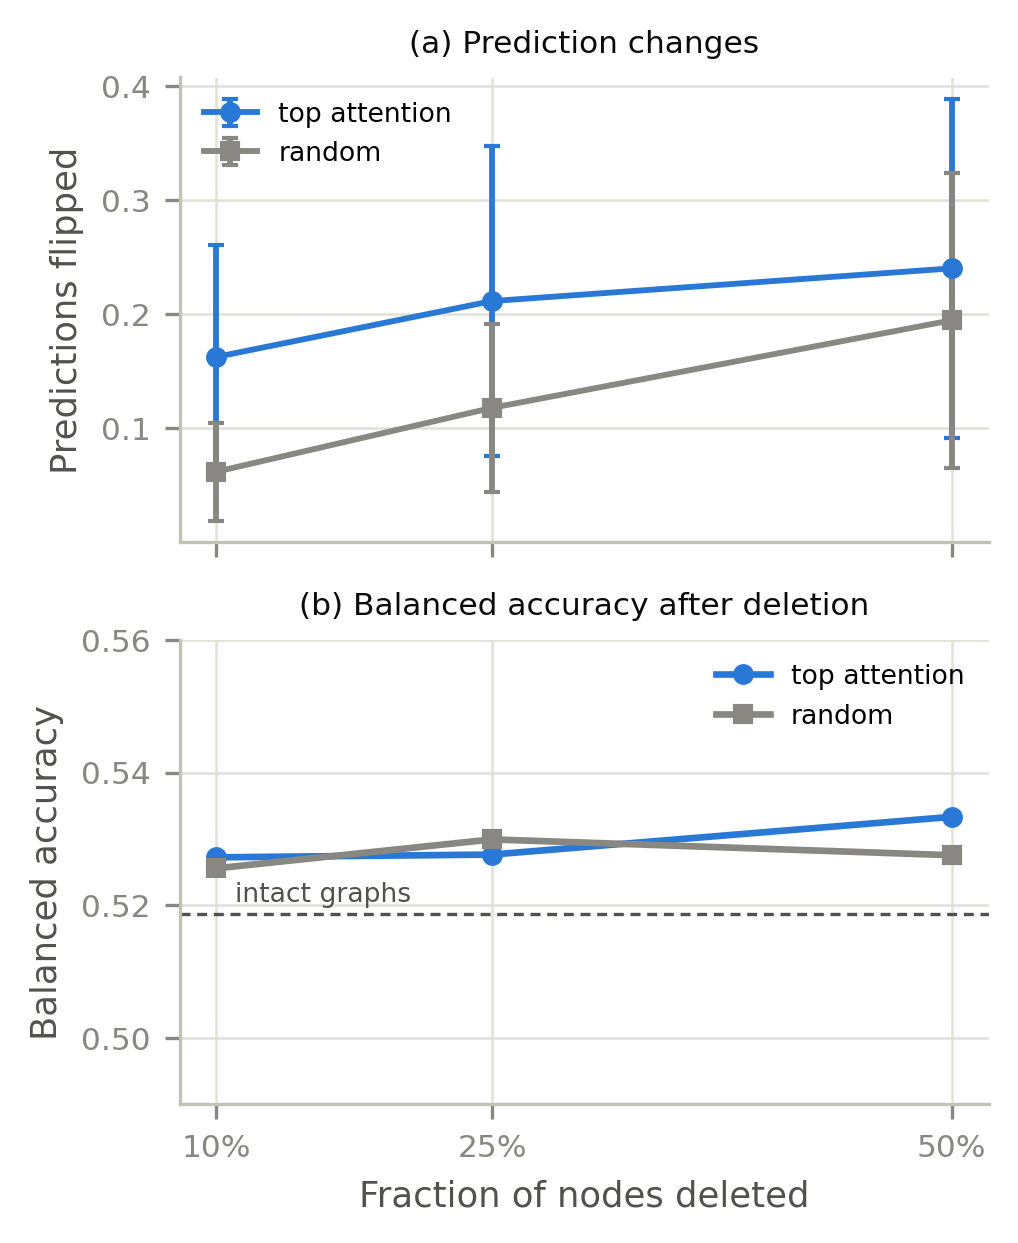
\includegraphics[width=\columnwidth]{figs/r_attention.png}
\caption{Attention faithfulness test on up to 2,000 test graphs per fold (seed-0 GAT).
(a) Fraction of predictions that change when the top-attention or random nodes are
deleted (mean $\pm$ standard deviation over folds); (b) balanced accuracy after
deletion, with the intact graphs for reference.}
\label{fig:attention}
\end{figure}

\subsection{Detector settings and the random-split gap (RQ3)}\label{sec:res-sens}
\paragraph{Peak detector.} Raising the prominence threshold removed more Elephant than
Giraffe windows (Figure~\ref{fig:detector}a): at $\rho=0.25$, 48.1\% of Elephant and
56.1\% of Giraffe windows kept two or more peaks, against 82.3\% and 80.8\% at the
default. The detector setting thus changes the class composition of the cohort, which is
a source of bias whenever cohorts are not matched across models. At $\rho=0.5$ too few
Giraffe windows remained at some stations to form valid folds. Balanced accuracy of
XGBoost on the pooled peak features stayed between 0.526 and 0.541 across the valid
settings (Figure~\ref{fig:detector}b), and a longer minimum separation, which reduced
the mean graph from 64.5 to 23.5 nodes, made no difference. The default detector is
therefore not responsible for the weak results of the peak-based models.

\begin{figure}[pos=t]
\centering
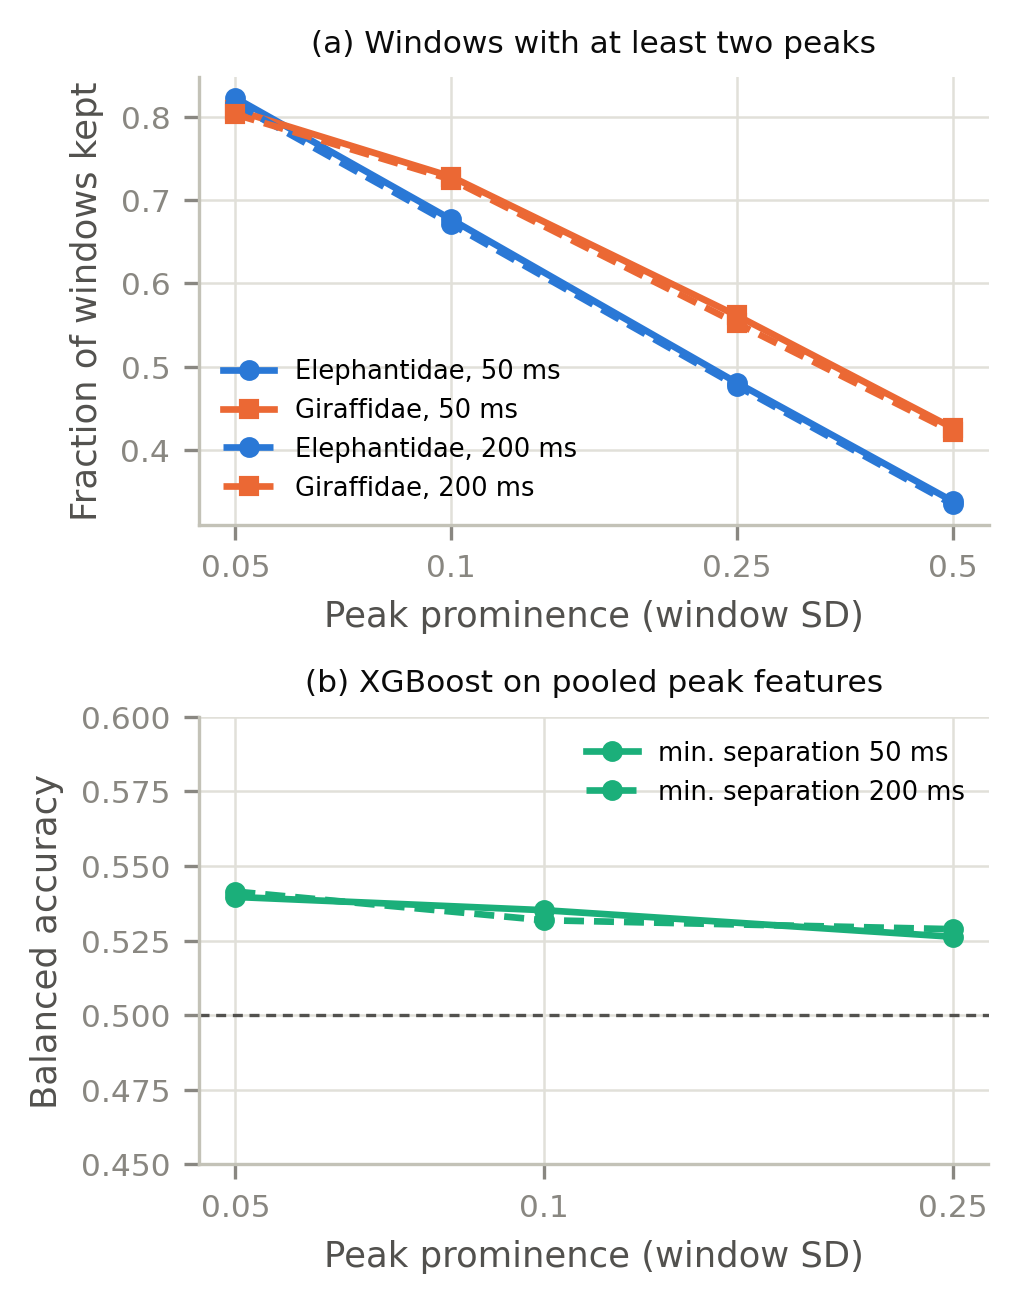
\includegraphics[width=\columnwidth]{figs/r_detector_sweep.png}
\caption{Peak-detector sensitivity. (a) Fraction of windows of each class with at
least two peaks, by prominence and minimum separation; (b) station-held-out balanced
accuracy of XGBoost on the pooled peak features. Prominence 0.5 left some folds without
Giraffe validation windows and is not scored.}
\label{fig:detector}
\end{figure}

\paragraph{Earlier random-split results.} Figure~\ref{fig:original} compares the earlier
results, obtained with a random window-level split and test-set selection, with the
station-held-out benchmark. The flexible classical models lost most: XGBoost fell from
0.888 to 0.590, gradient boosting from 0.744 to 0.542, the SVM from 0.710 to 0.561 and
7-NN from 0.671 to 0.526, consistent with models that can match near-duplicate windows
benefiting most from leakage. The random forest (0.663 to 0.553), logistic regression
(0.655 to 0.603) and the GAT (0.585 to 0.559) lost less.
The ANN improved (0.485 to 0.551) because the benchmark allowed all three components and
validation-based early stopping. The two evaluations also differ in cohort, selection
and tuning, so this comparison measures the combined effect of the protocol, not of the
split alone; the direct random-split control (Section~\ref{sec:random-method}) isolates
the split. % TODO: report the control here.

\begin{figure}[pos=t]
\centering
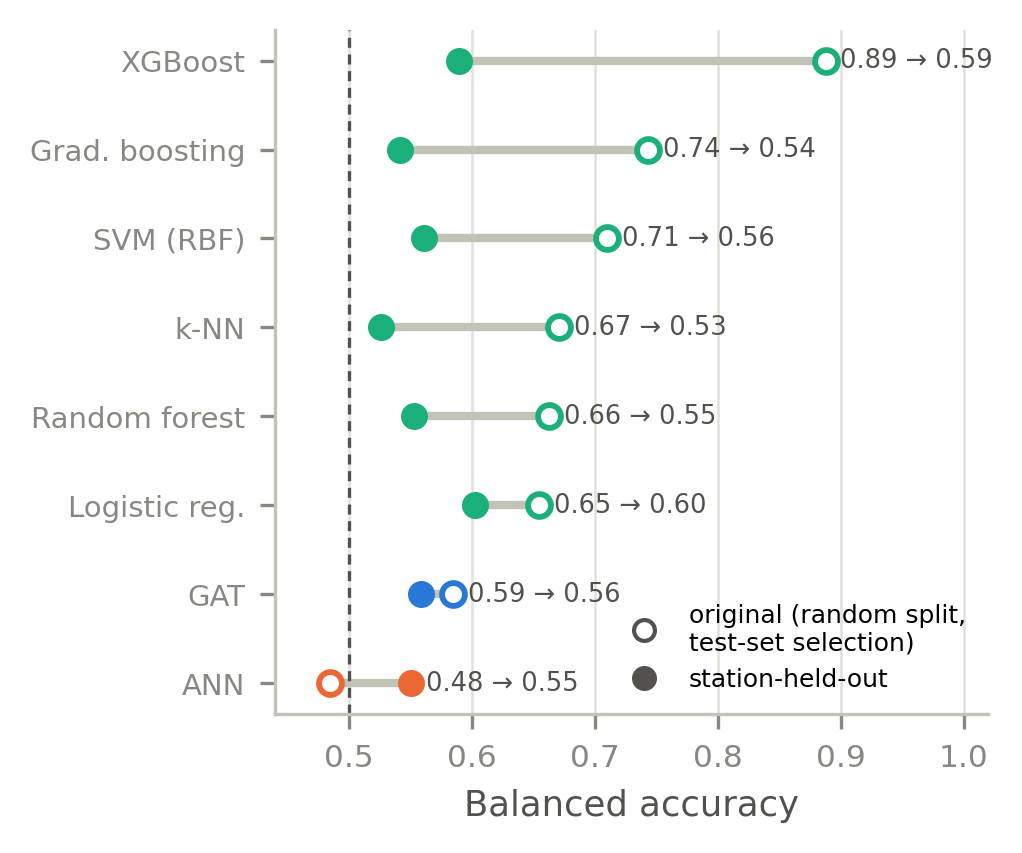
\includegraphics[width=\columnwidth]{figs/r_original_vs_controlled.png}
\caption{Balanced accuracy reported by the earlier random-split experiments with
test-set selection (open) and in the station-held-out benchmark (filled).}
\label{fig:original}
\end{figure}

\subsection{Edge-device cost (RQ4)}\label{sec:res-edge}
Table~\ref{tbl:edge} and Figure~\ref{fig:edge} give the measured footprints of the
fold-0 models. Against the 512\,KB flash budget, the GAT (112\,KB FP32, 89\,KB INT8),
feature MLP (13\,KB INT8), KAN (59\,KB), GCN (29\,KB INT8, of which 16\,KB is the stored
$64\times64$ normalised adjacency) and 1D-CNN (377\,KB) fit, as do logistic regression
(29 parameters) and XGBoost once its trees are written as C arrays (1,992 splits and
2,292 leaves; 26.5\,KB, against 339\,KB for the serialised Python object). The ANN does
not fit: even its smallest selected configuration needs 2.19\,MB in FP32 and 559\,KB
after INT8 quantisation, and the configurations selected in the other folds are three to
six times larger. The SVM, $k$-NN and random forest store support vectors, the training
set or deep trees (5.0--31\,MB) and do not fit.

\begin{table*}[width=.98\textwidth,cols=8,pos=t]
\caption{Measured footprint of the fold-0, seed-0 model of each family. Sizes are
serialised files (KB $=1024$ bytes); INT8 uses PyTorch dynamic quantisation, which
quantises linear layers only. Times are host-CPU medians with one thread over 200 test
windows; they rank models but are not device latencies. Budget: 512\,KB of flash.}
\label{tbl:edge}
\footnotesize
\begin{tabular*}{\tblwidth}{@{}l@{\extracolsep{\fill}}lrrrrrl@{}}
\toprule
Model & Fold-0 configuration & Params & FP32 (KB) & INT8 / C (KB) & Pre.\ (ms) & Infer.\ (ms) & Fits flash \\
\midrule
GAT & $H=64$, $K=2$, raw & 26,882 & 112.1 & 89.1 & 1.46 & 1.50 & yes (sparse kernel) \\
ANN & X, $H=256$ & 558,466 & 2,189.7 & 558.9 & 0.04 & 0.21 & no \\
Feature MLP & $H=64$ & 4,194 & 22.2 & 12.8 & 0.54 & 0.12 & yes \\
1D-CNN & $c=32$ & 94,210 & 377.0 & 376.1 & 0.06 & 0.70 & yes \\
KAN & 32--16 & 13,120 & 58.8 & 58.8 & 0.65 & 0.92 & yes (spline tables) \\
GCN & 21 statistics & 3,746 & 36.6 & 28.6 & 0.26 & 0.57 & yes \\
XGBoost & depth 3, lr 0.1 & --- & 339.3$^{a}$ & 26.5$^{b}$ & 0.53 & 0.42 & as C arrays \\
Logistic reg. & $C=1$ & 29 & 0.9$^{a}$ & --- & 0.53 & --- & yes \\
Random forest & depth 20 & --- & 31,310$^{a}$ & --- & 0.53 & 39.66 & no \\
\bottomrule
\end{tabular*}
\par\smallskip\raggedright\footnotesize $^{a}$ Serialised Python object.
$^{b}$ Trees as flat C arrays, computed from the node counts.
\end{table*}

\begin{figure}[pos=t]
\centering
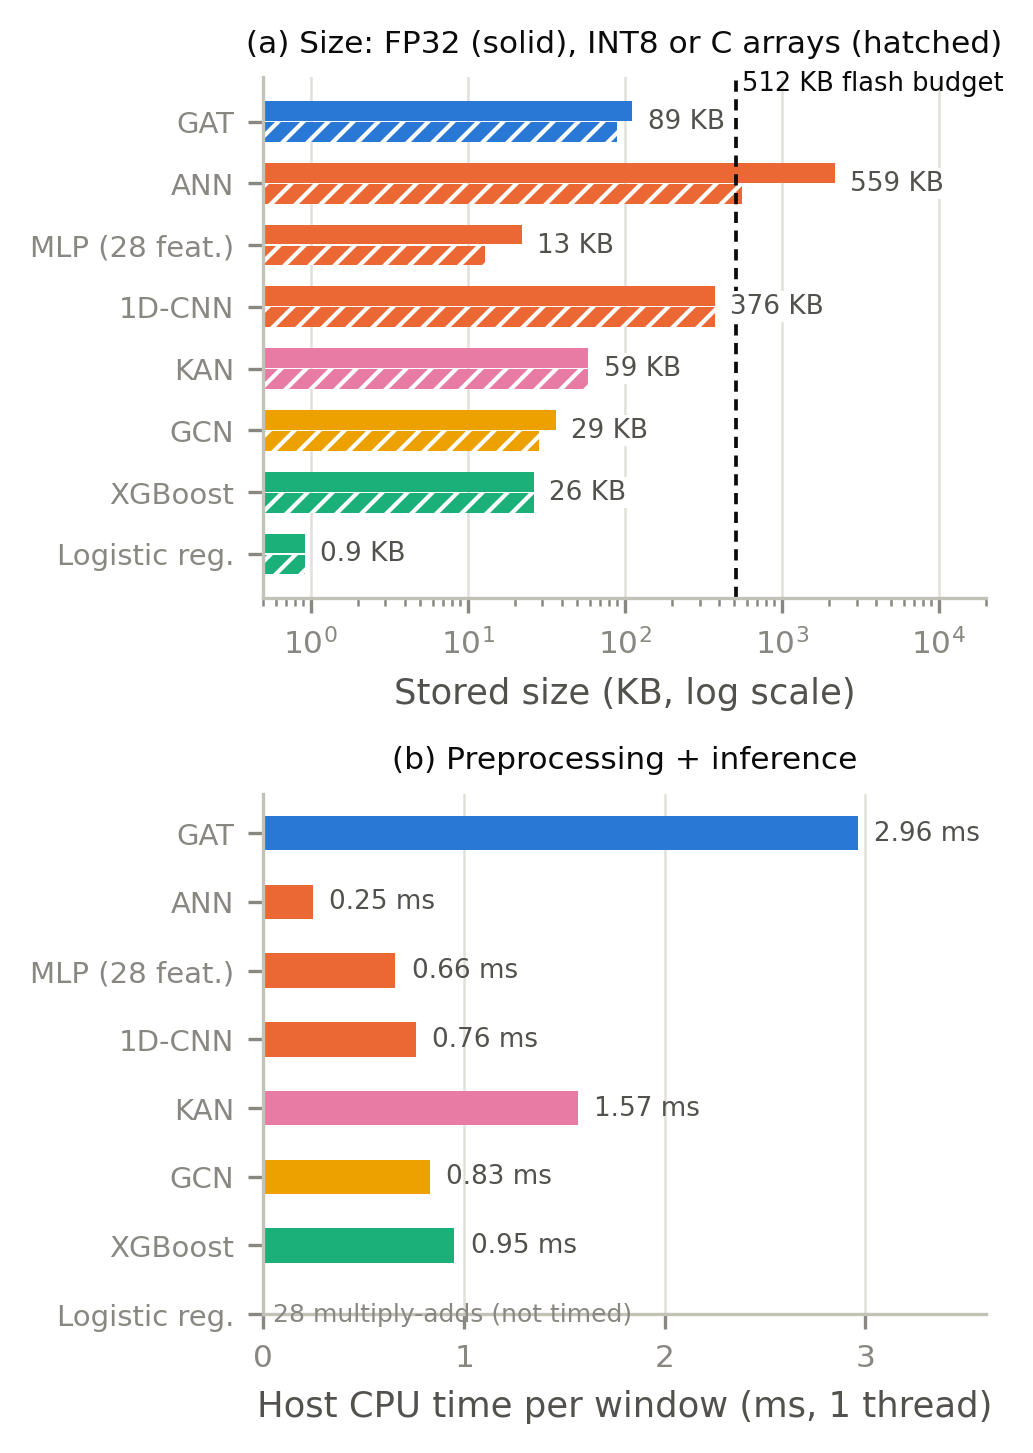
\includegraphics[width=\columnwidth]{figs/r_edge_profile.png}
\caption{Measured footprint of the fold-0 models. (a) Stored size in FP32 (solid) and
after INT8 quantisation or, for XGBoost, as C arrays (hatched), on a logarithmic axis; the
dashed line marks the 512\,KB flash budget. (b) Host-CPU time per window for
preprocessing plus inference (one thread).}
\label{fig:edge}
\end{figure}

\paragraph{What a graph model costs on a microcontroller.} On the host the GAT was the
slowest network: building the graph took 1.46\,ms (95th percentile 6.0\,ms, because cost
grows with the number of peaks) and inference 1.50\,ms, against 0.25--1.57\,ms for the
other networks and 0.95\,ms for XGBoost including feature extraction. On the device the
graph also sets the memory. With $E(N)=7N-2$ edges plus $N$ self-loops, the largest
simultaneously live buffers (per-head node features and one attention coefficient per
edge and head) need 36\,KB for the selected fold-0 configuration ($H=64$, $K=2$) at the
mean graph of 64.5 nodes and 84\,KB at 150 nodes, within the 200\,KB working-memory
budget, and inference needs 1.4 and 3.3 million MACs. These figures assume a sparse,
edge-list implementation. Padding every graph to 150 nodes and computing dense attention,
the usual route on microcontrollers, would need a $150\times150\times K$ attention matrix
plus node features, about 251\,KB for $K=2$ and 502\,KB for $K=4$, which exceeds the
budget. Standard microcontroller runtimes provide dense and convolutional operators but
no graph message passing, so the GAT would need a hand-written sparse kernel, on-device
peak detection and a nearest-neighbour search ($N^2F=180{,}000$ MACs at 150 nodes) before
inference. The feature-based models need only the 28 statistics, which are linear in the
2,048 samples, and a small model.

\section{Discussion}\label{sec:discussion}

\paragraph{Station shift dominates.} The central finding is that, on stations not seen
during training, every model in this study separated Giraffidae from Elephantidae only
weakly (balanced accuracy at most about 0.60, AUROC at most 0.62), and that the choice of
held-out stations changed scores far more than the choice of model. Validation and test
stations disagreed so strongly that model selection on validation stations could not
anticipate test performance. Two explanations are compatible with the data. First,
station-specific factors such as coupling, local geology, background noise and the
distance distribution of sightings may dominate the class signal in 10-s windows.
Second, the class signal may be weak at the distances in this release (up to 150\,m),
where \citet{szenicer2022} also reported their lowest scores. Either way, the earlier
high scores reflected recognition of recordings resembling those seen in training rather
than of species, and comparisons of model families on random splits of these data are
not informative about deployment.

\paragraph{Relation to prior work.} \citet{szenicer2022} reported balanced accuracy of
about 0.73 at 150\,m for elephant-versus-other detection with time-ordered splits, and
lower accuracy on held-out stations; \citet{steinmann2025} reported 0.77 at 150\,m for
four species. Our task (Giraffidae versus Elephantidae from 10-s windows of an 11--150\,m
release) and our protocol (whole stations held out, no time information) differ from
both, and our models use no spectrogram or pretrained representation. Our numbers are
therefore not a ranking against theirs but a warning that held-out-station performance
on this release is much lower than window-level splits suggest.

\paragraph{Graph models.} Under a fair protocol the peak-graph GAT was neither better nor
clearly worse than the classical and neural baselines, and nothing in the ablations
attributes value to the graph structure: message passing between peaks helped relative
to no edges, but random connections served as well as temporal or feature-space ones,
and a graph-free model on the same peak information performed similarly. The GCN on
fixed segments was weaker still. Given the engineering cost of graph inference on a
microcontroller, a graph representation of envelope peaks is not justified for this task
on the present evidence. Graphs whose nodes correspond to footfalls or to stations in an
array, as used for localisation \citep{reinwald2021}, may behave differently and remain
untested.

\paragraph{Simple models suffice for now.} Logistic regression on 28 features matched the
best models at a cost of 29 parameters, and XGBoost and a 13\,KB feature MLP were close
behind. Low-capacity models may be less able to fit station-specific structure, which
would explain why they do not lose to larger ones under station shift. For deployment,
these models fit the ESP32-S3 with large margins and need no graph construction.

\paragraph{Limitations.} (i) No model was executed on the microcontroller; host
latencies rank models but do not predict device latency or energy, and INT8 sizes come
from dynamic quantisation of linear layers only. (ii) With ten stations, five folds of
one to three stations each give noisy fold estimates. (iii) The release lacks sighting
and time identifiers, so windows from one passage at one station can still fall into
both the training and validation parts of the inner split; this affects selection, not
the held-out test stations. (iv) Thresholds were fixed at 0.5 and not calibrated per
station. (v) Grids were small and comparable rather than exhaustive, and the ablations
used one seed. (vi) Only the binary Elephantidae--Giraffidae task was studied; the
rarer families have too few windows at most stations for station-held-out evaluation.

\paragraph{Future work.} The results point to domain generalisation rather than new
architectures: station-wise normalisation or adaptation, representations that are
invariant to coupling and site response (for example spectral ratios or
spectrogram-based pretraining), distance-stratified evaluation, and data from more
stations and sites. On-device measurement of the feature-based models and of a sparse
GAT kernel would complete the edge assessment.

\FloatBarrier
\section{Conclusions}\label{sec:conclusion}
We compared thirteen classifiers from five families for separating Giraffidae from
Elephantidae in seismic windows, under a protocol that holds out whole recording
stations and tunes every model on validation stations only.
\begin{itemize}
\item \textbf{RQ1.} All classifiers were weak on unseen stations (pooled balanced
accuracy 0.526--0.603, AUROC at most 0.621). Logistic regression, XGBoost, a 1D-CNN and
a feature MLP formed an indistinguishable leading group; the GAT (0.559), KAN (0.544)
and GCN (0.528) did not improve on them. Accuracy ranked the worst model by balanced
accuracy first.
\item \textbf{RQ2.} The peak graph's topology added no measurable information: random
edges matched structured edges and a graph-free model on the same peak features
performed similarly. Attention marked influential nodes but not class evidence that
transferred.
\item \textbf{RQ3.} Hyperparameters and detector settings mattered little; the held-out
stations mattered most, and validation scores did not predict test scores ($r=-0.02$).
Random window-level splits with test-set selection had inflated XGBoost's balanced
accuracy from 0.590 to 0.888.
\item \textbf{RQ4.} The GAT, GCN, KAN, feature MLP, 1D-CNN, logistic regression and
XGBoost (as C arrays) fit a 512\,KB flash budget; the raw-waveform ANN, SVM, $k$-NN and
random forest do not. The GAT additionally needs a sparse graph kernel and on-device
graph construction.
\end{itemize}
For seismic wildlife classification on this release, generalisation across stations,
not the choice among these model families, is the problem to solve, and evaluations
should hold out stations or time blocks.

\FloatBarrier

\section*{Data availability}
The SeisSavanna dataset is publicly available from its authors \citep{szenicer2022}.
The benchmark script, its configuration, all per-run results with training histories,
the out-of-fold predictions and the scripts that draw every figure will be made
available. % TODO: add repository URL.

\section*{Acknowledgements}
We thank the creators of the SeisSavanna dataset for making their recordings and
labels publicly available. % TODO: add further acknowledgements.

\FloatBarrier
\bibliographystyle{cas-model2-names}
\bibliography{cas-refs}

\end{document}
